\documentclass{article}
\usepackage[T1]{fontenc}  
\usepackage[utf8]{inputenc}  
\usepackage[spanish]{babel}  
\usepackage{amsmath,amssymb}
\usepackage{amsthm}
\usepackage[affil-it]{authblk}
\usepackage{hyperref}
\usepackage{gensymb}
\usepackage[export]{adjustbox}
\usepackage[center]{caption}
\usepackage{graphicx}
\usepackage{biblatex}
\hypersetup{
    colorlinks=true,
    linkcolor=blue,
    filecolor=magenta,      
    urlcolor=cyan,
    pdftitle={Overleaf Example},
    pdfpagemode=FullScreen,
    }

\addbibresource{biblio.bib}

\author{Luis Lucas García}
\affil{Universidad de Alicante - Facultad de Ciencias - Grado en Física - Técnicas experimentales II - Grupo L1}
\title{Experimento de Franck - Hertz}
\date{\today}

\begin{document}
\maketitle

\begin{abstract}
El experimento de Franck-Hertz les valió el nóbel en 1925 y permite observar la naturaleza cuántica de la realidad. En este experimento se pretende observar la cuantización de los niveles de energía de los átomos. Para ello utilizaremos un montaje en el que mediante la emisión de termoelectrones estimularemos el material para observar la ionización de los átomos. En esta práctica se consiguen obtener adecuadamente los valores de la energía de excitación para el mercurio y el neón con un error relativamente bajo.
\end{abstract}

\tableofcontents

\section{Fundamento teórico}

En este experimento trabajaremos con dos elementos distintos de la tabla periódica: el mercurio y el neón. Las configuraciones electrónicas de dichos elementos son:

$$
\begin{array}{cc}
Hg (Z = 80) = [Xe]4f^{14} 5d^{10} 6s^2 & Ne (Z = 10) = [He] 2s^2 2p^6
\end{array}
$$

En nuestro caso únicamente consideraremos los electrones más exteriores, es decir, los electrones de la capa de valencia. Ya que los electrones internos tendrán una atracción al núcleo muy fuerte mientras que los externos tienen esta atracción apantallada por el resto de electrones.

Para el caso del mercurio, podemos encontrar el estado de los electrones de valencia. En este caso como $l_1 = l_2 = 0$ entonces no queda otra que $L = 0$ y el valor $S = 0, 1$. Ahora bien, como L es simétrico sólo queda que S sea antisimétrico por lo que tenemos el mercurio en un estado fundamental $^1S_0$. Los estados excitados del mercurio serán $^3P_0$, $^3P_1$ y $^3P_2$. También existe un estado singlete excitado $^1P_1$. Nos vamos a centrar en la excitación al estado $^3P_1$ pues es la que experimentalmente más se observa.

En un experimento realizado por alumnos de otra universidad obtienen unos valores experimentales de la energía de excitación $E_a = 4.80 \pm 0.11 eV$ \cite{UnivBonn}.

Para el neón, la excitación más probable es a los estados 3p. La energía de ionización tiene un valor de $21.56eV$ donde ignoramos el error del artículo pues es mucho menor al que nosotros consideramos. Así nos queda que la diferencia de energía entre estos estados excitados y el estado fundamental está entre los $18.4eV$ y los $19.0eV$\cite{Neon}. Cabe notar que también puede suceder una excitación al estado 3s pero es menos probable.

\begin{figure}[h!]
\begin{center}
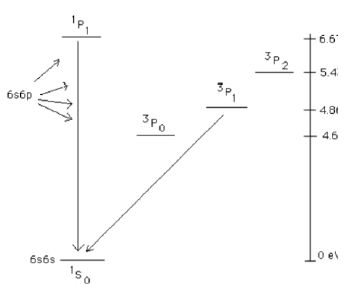
\includegraphics[max width=0.49\linewidth]{HgTeo.png}
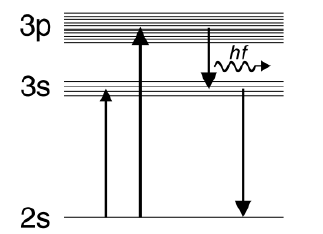
\includegraphics[max width=0.49\linewidth]{NeTeo.png}
\caption{Diagramas de las transiciones para el mercurio (izquierda) y el neón (derecha).}
\end{center}
\end{figure}

Siempre que se emiten energía lo hace en forma de fotones, que por las expresiones de Planck tienen la misma energía que la diferencia entre los dos estados y la frecuencia viene dada por $E = h \nu$. Para las transiciones del mercurio $\lambda = 254nm$ mientras que las del neon entran en el visible. La longitud de onda dada por una transición se puede encontrar como:

\begin{equation}
\lambda = \frac{hc}{\Delta E}
\label{eq:lambda}
\end{equation}

\section{Desarrollo experimental}

\subsection{Dispositivo para el mercurio}

En el caso del mercurio contamaos con un dispositivo como el que aparece en la figura (\ref{fig:FHHg}).

\begin{figure}[h!]
\begin{center}
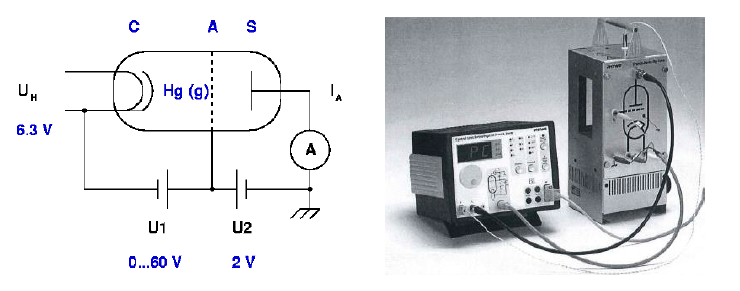
\includegraphics[max width=\linewidth]{FHHg.png}
\caption{Diagrama del dispositivo de Franck-Hertz.}
\label{fig:FHHg}
\end{center}
\end{figure}

Este dispositivo consta de varias partes que aparecen en la imagen.

\begin{enumerate}
\item \textbf{C - Cátodo emisor de termoelectrones:} esta parte emite electrones en forma de efecto termoiónico. La temperatura permite a los electrones superar la energía de la función de trabajo del material y liberarse. \cite{thermoIonic}. La tensión alterna que pasa por aquí es $U_H = 6.3 V$.
\item \textbf{A - Ánodo en forma de rejilla:} se encarga de acelerar los electrones emitidos. Aplicaremos una diferencia de potencial variable $U_1$ entre C y A que va a definir la energía de los electrones, recordemos que en un potencial $E = eU_1$.
\item \textbf{S - Electrodo colector:} se encarga de recoger los electrones con la energía suficiente para llegar a él, midiendo la corriente $I_A$. Podemos aplicar un potencial de frenado $U_2$ que nos permite obtener los electrones con mayor velocidad para observar más claramente las gráficas.
\end{enumerate}

Dentro del tubo encontramos gas de mercurio, los electrones emitidos pueden colisionar con estos electrones, perdiendo energía. Si la teoría cuántica es cierta, únicamente perderán energía los electrones que tengan energía suficiente para excitar los átomos de mercurio. Los que tengan una energía menor simplemente harán una colisión elástica sin perder energía, pues no tendrán ninguna acción sobre los electrones de valencia del mercurio.

Es claro que, si un electrón lleva una energía mayor a la energía de excitación del mercurio, tras una colisión inelástica llevará una energía $eU_1 - E_a$. Sin embargo, si después de la colisión esta energía sigue siendo suficiente, este electrón podría volver a colisionar con otro átomo de mercurio, causando otra emisión y generando, en general, una energía final $eU_1 - nE_a$. Cuando los electrones tengan una energía suficiente para excitar los átomos de mercurio, el detector S detectará un mínimo de intensidad, pues llegan menos electrones con energía suficiente para vencer el potencial de frenado $U_2$.

Podemos caracterizar los potenciales $U_1$ en los que ocurrirán estos mínimos por la expresión:

\begin{equation}
U_{1, min} = n \frac{E_a}{e}
\label{eq:Ea}
\end{equation}

Para la mejor realización del experimento el tubo deberá estar entre 140ºC y 175ºC. El tubo estará calefactado para ello, de este modo haremos el recorrido libre medio menor a la distancia entre C y A. El dispositivo está conectado a un ordenador que nos permite controlar todas las cantidades a través de un programa.

Realizando las medidas obtenemos las gráficas de la figura (\ref{fig:medHg}).

\begin{figure}[h!]
\begin{center}
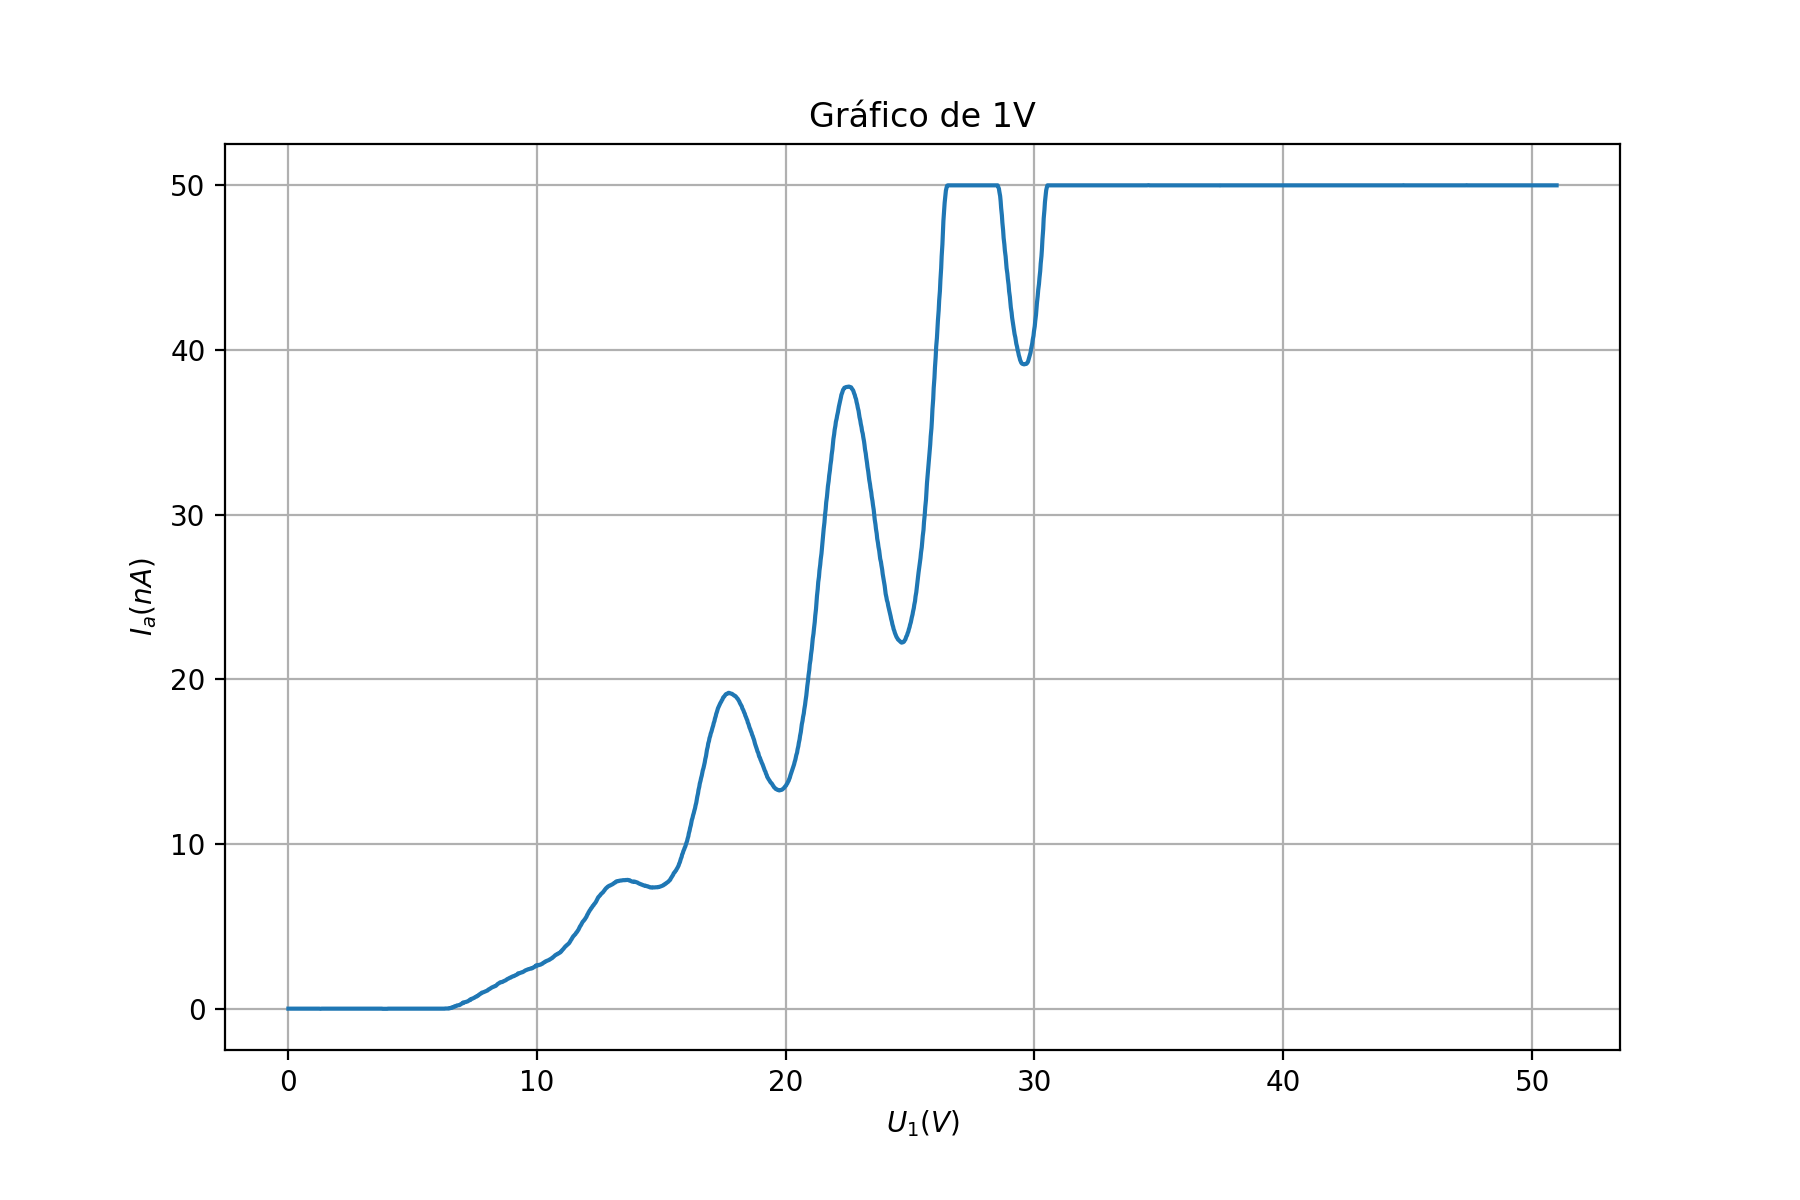
\includegraphics[max width=0.32\linewidth]{Hg Gráfico de 1V}
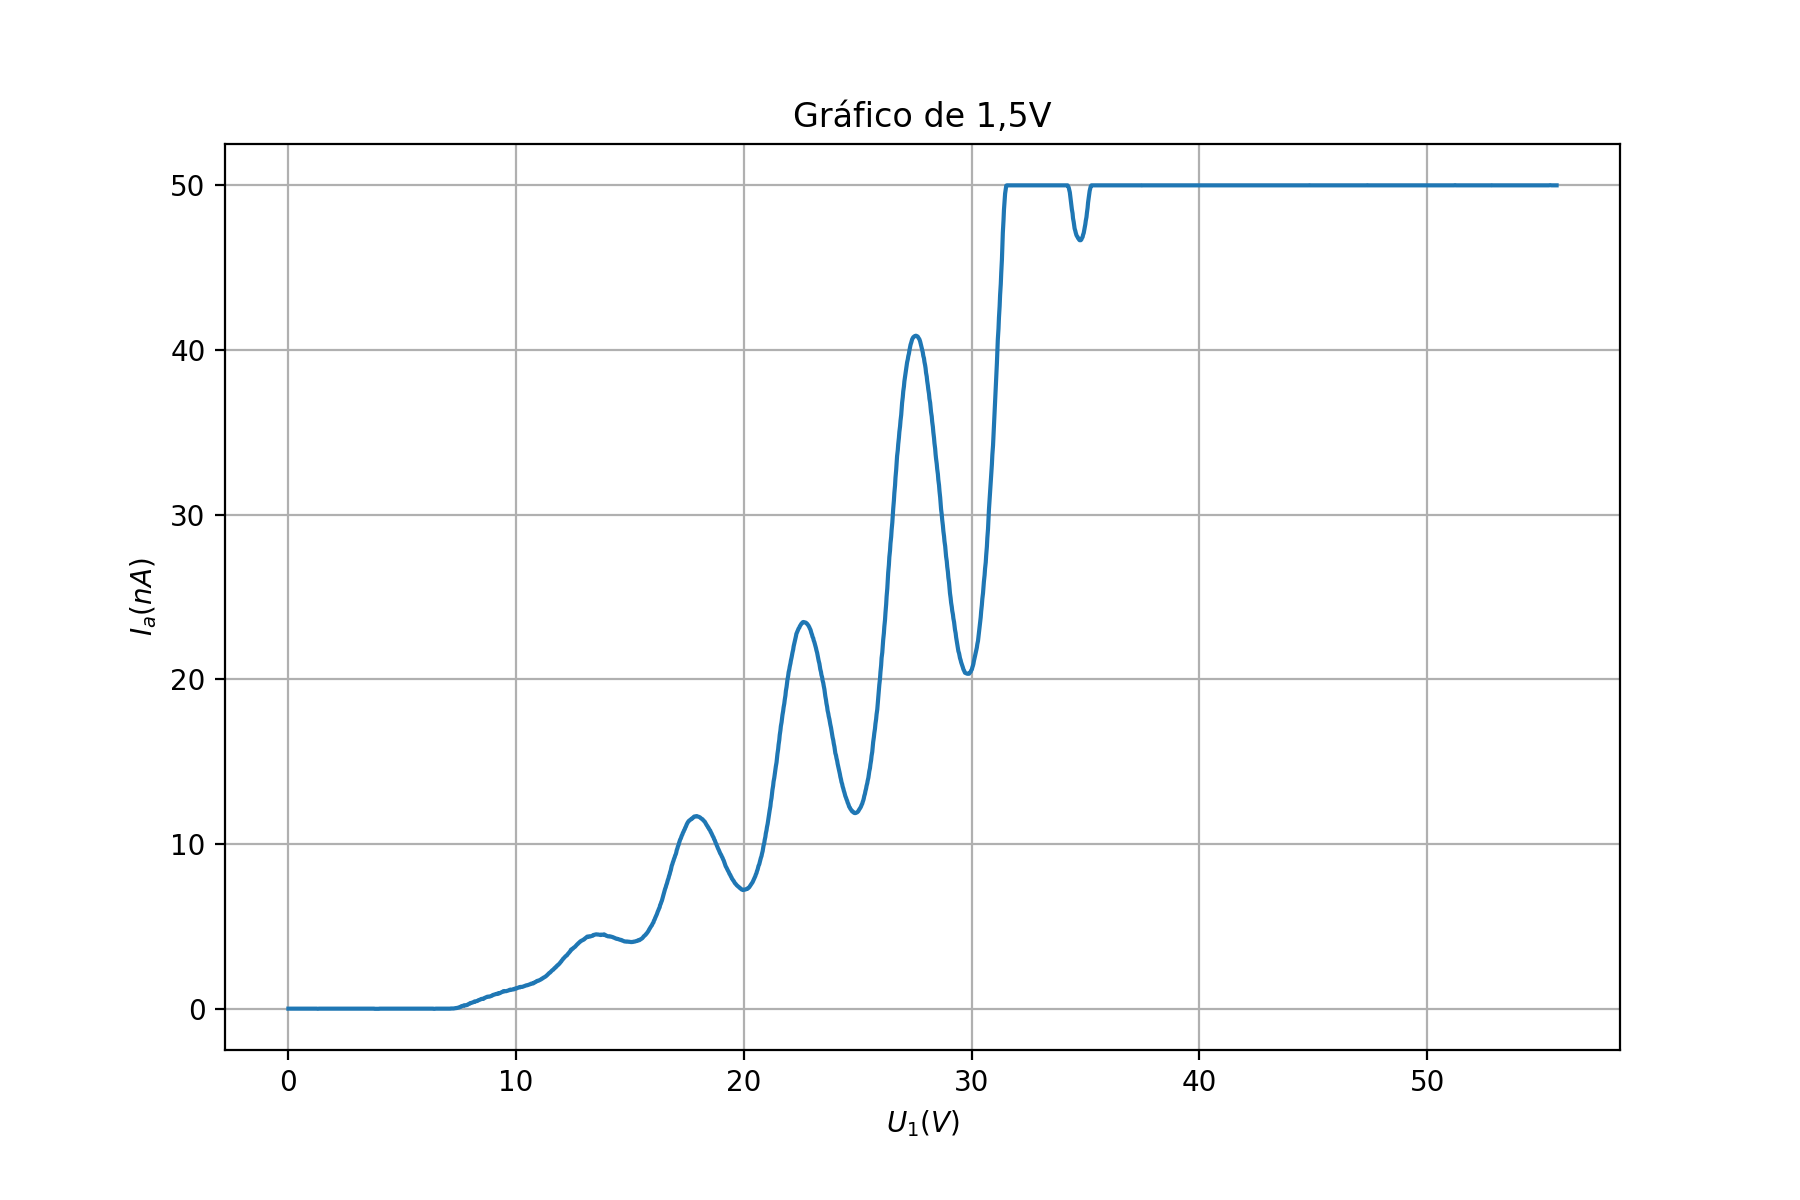
\includegraphics[max width=0.32\linewidth]{Hg Gráfico de 1,5V}
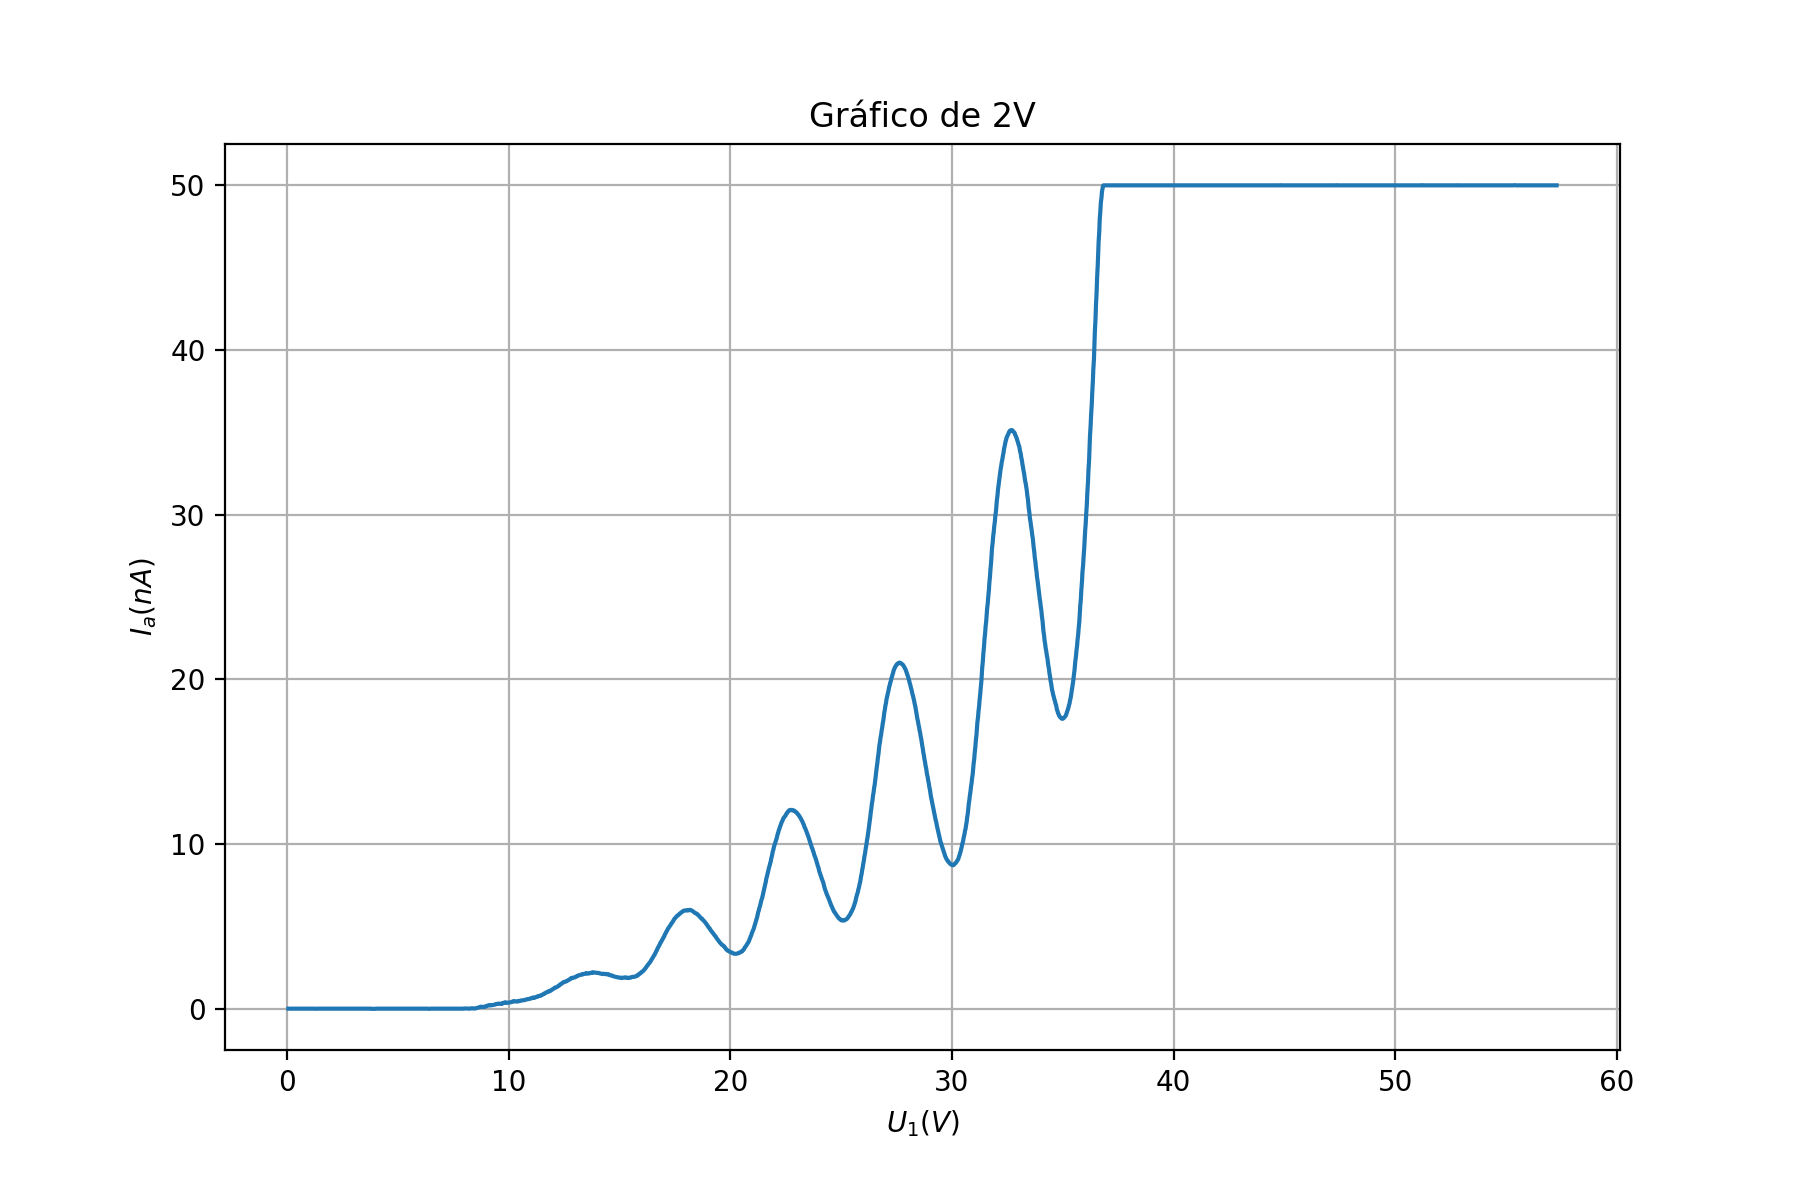
\includegraphics[max width=0.32\linewidth]{Hg Gráfico de 2V}
\caption{Gráficas obtenidas para un potencial de frenado de 1V, 1,5V y 2V respectivamente.}
\label{fig:medHg}
\end{center}
\end{figure}

También realizamos medidas variando la temperatura con el resto de parámetros estándar del programa de Phywe para un análisis que haremos en la siguiente sección. Las gráficas que obtenemos son las de la figura (\ref{fig:tempsHg}).

\begin{figure}[h!]
\begin{center}
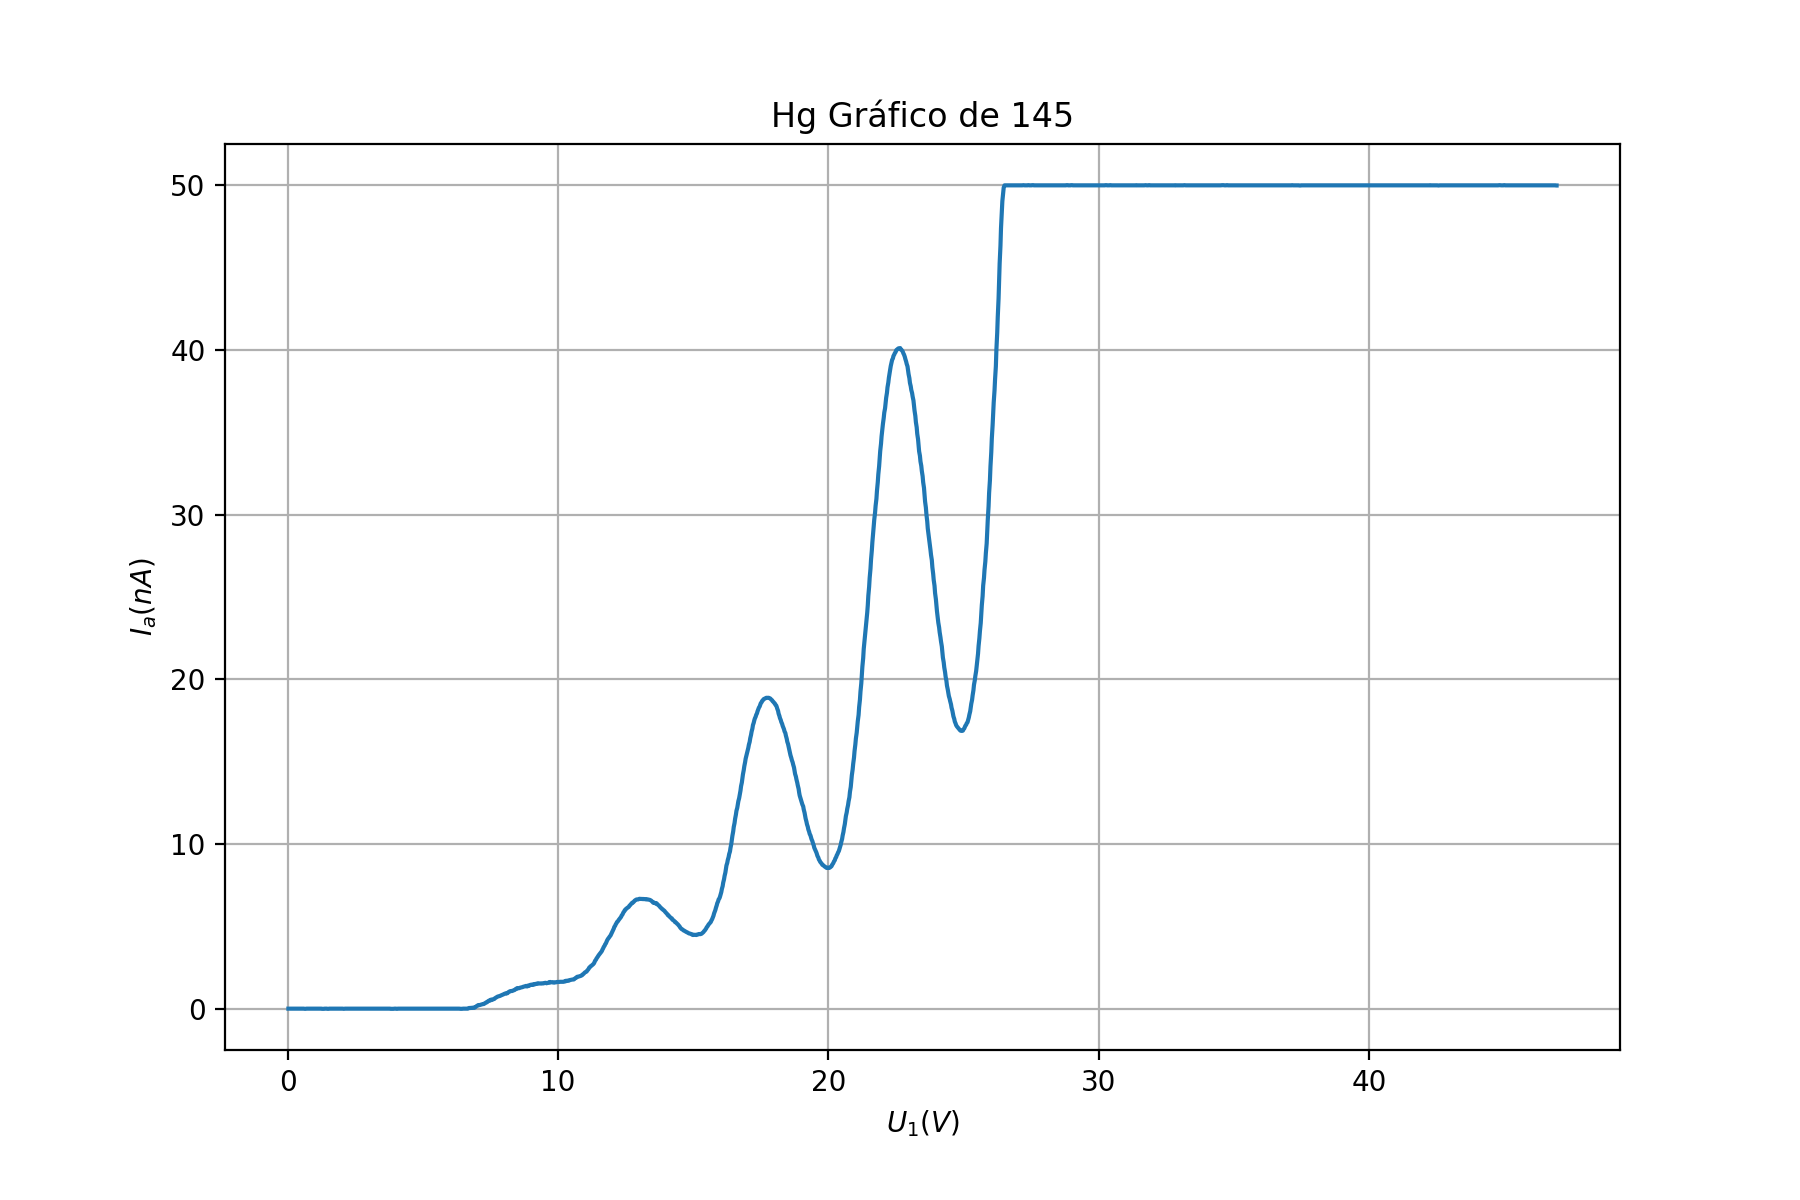
\includegraphics[max width=0.49\linewidth]{Hg Gráfico de 145}
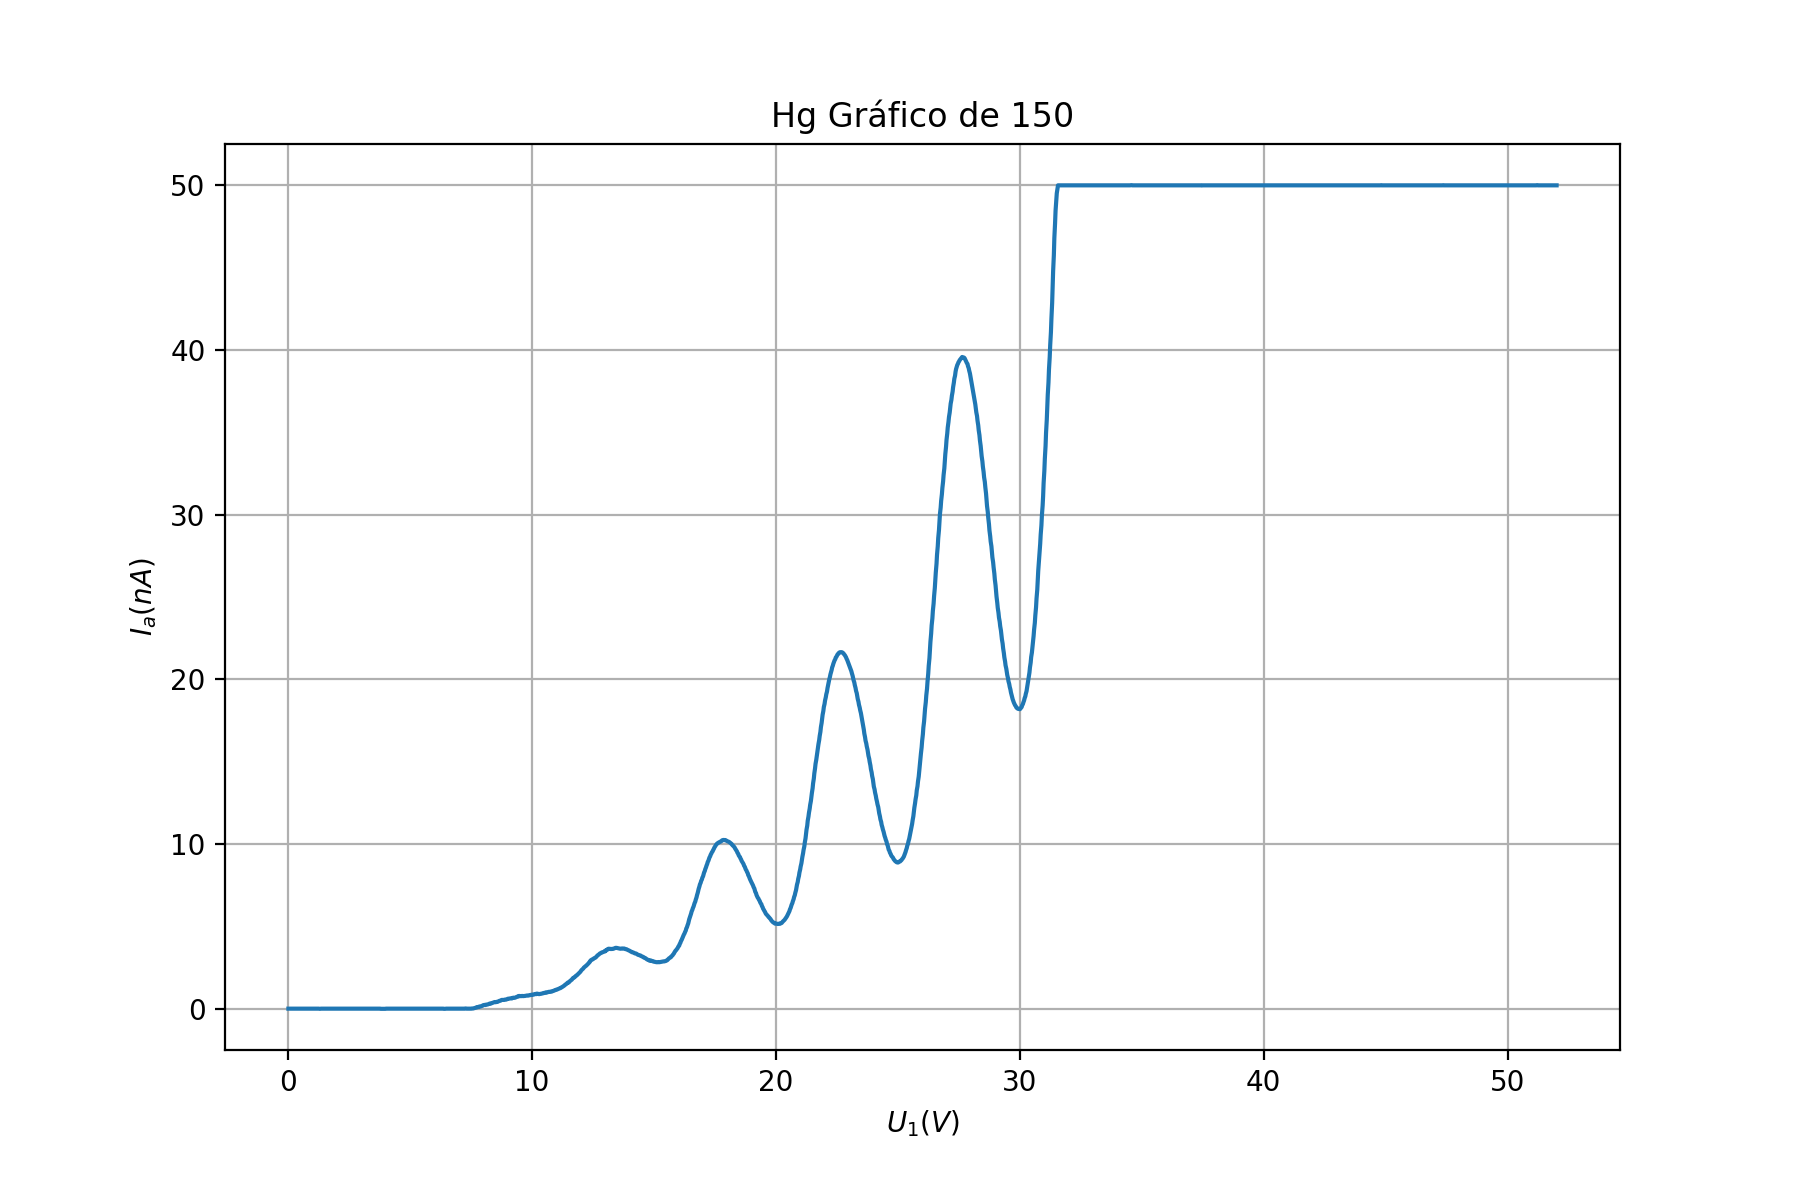
\includegraphics[max width=0.49\linewidth]{Hg Gráfico de 150}
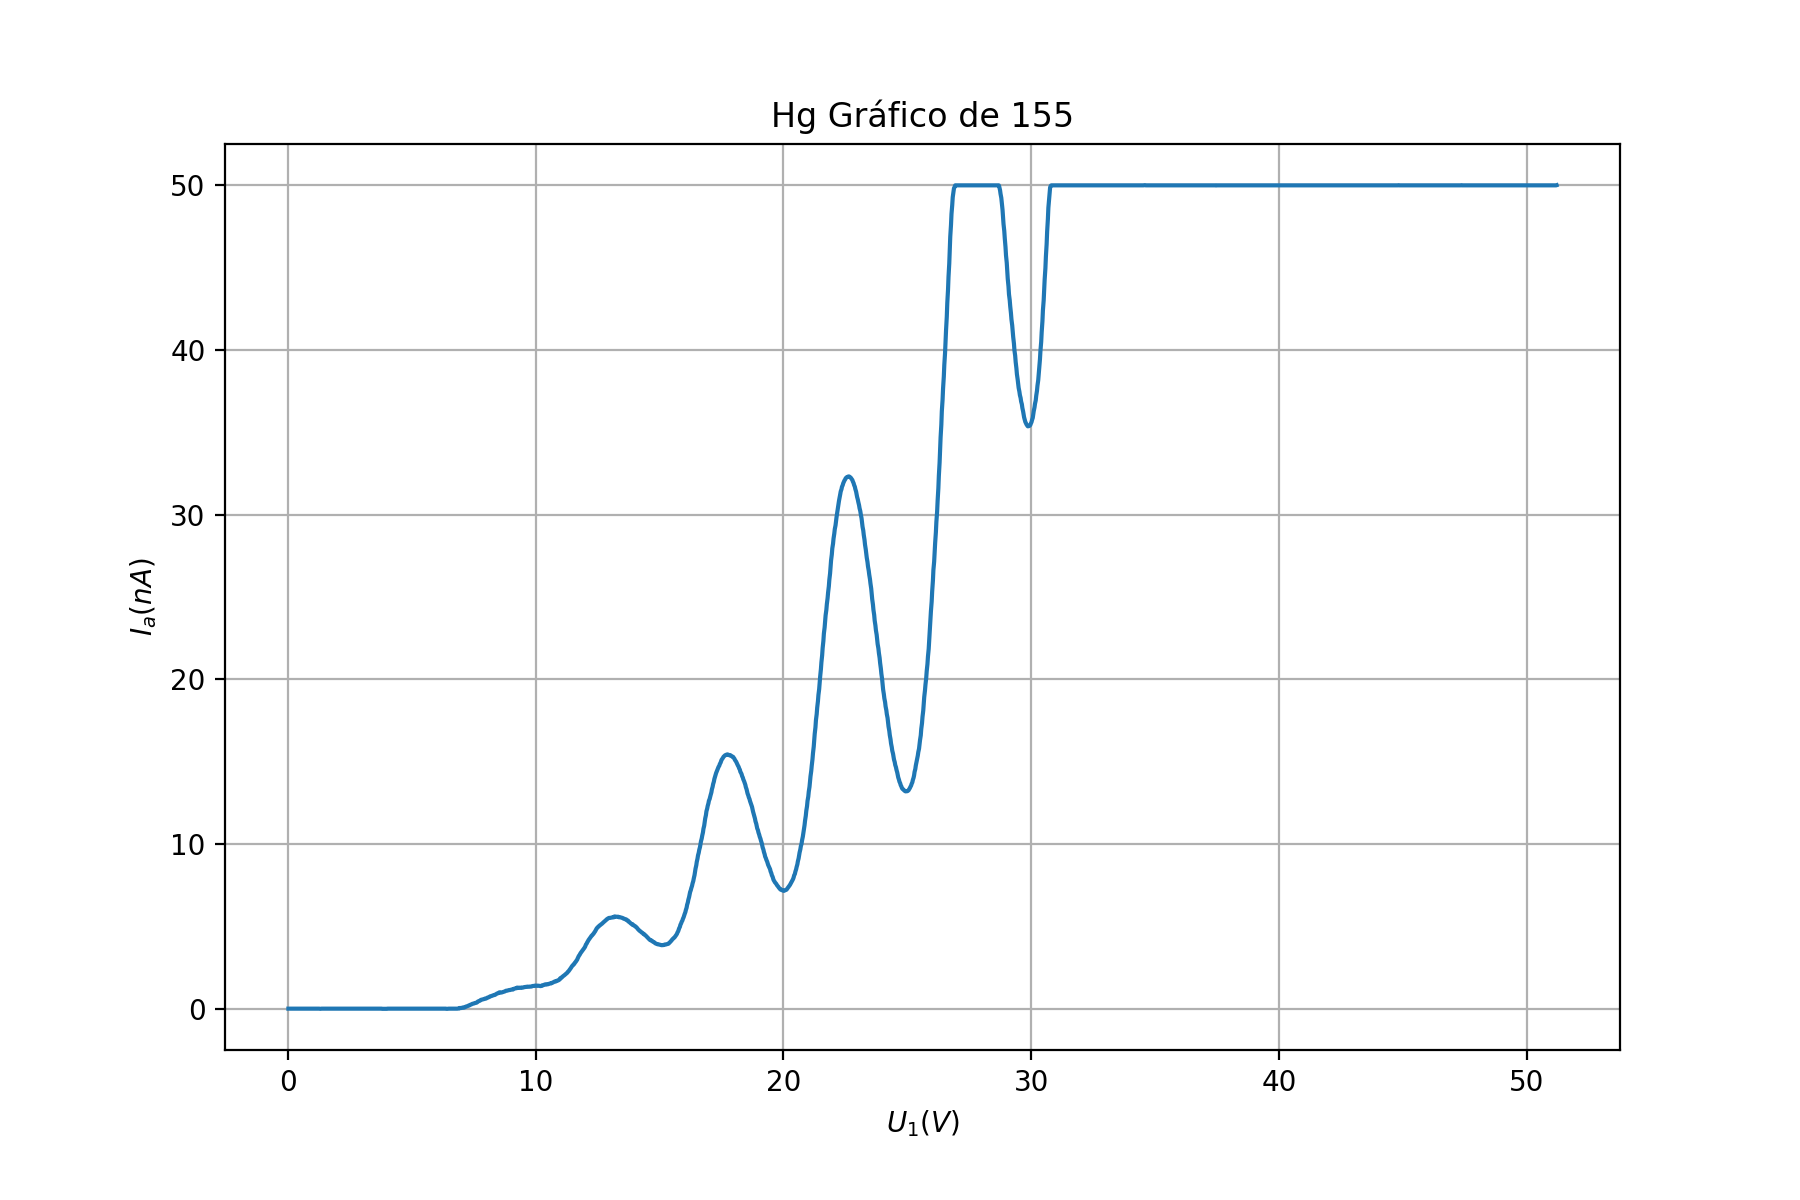
\includegraphics[max width=0.49\linewidth]{Hg Gráfico de 155}
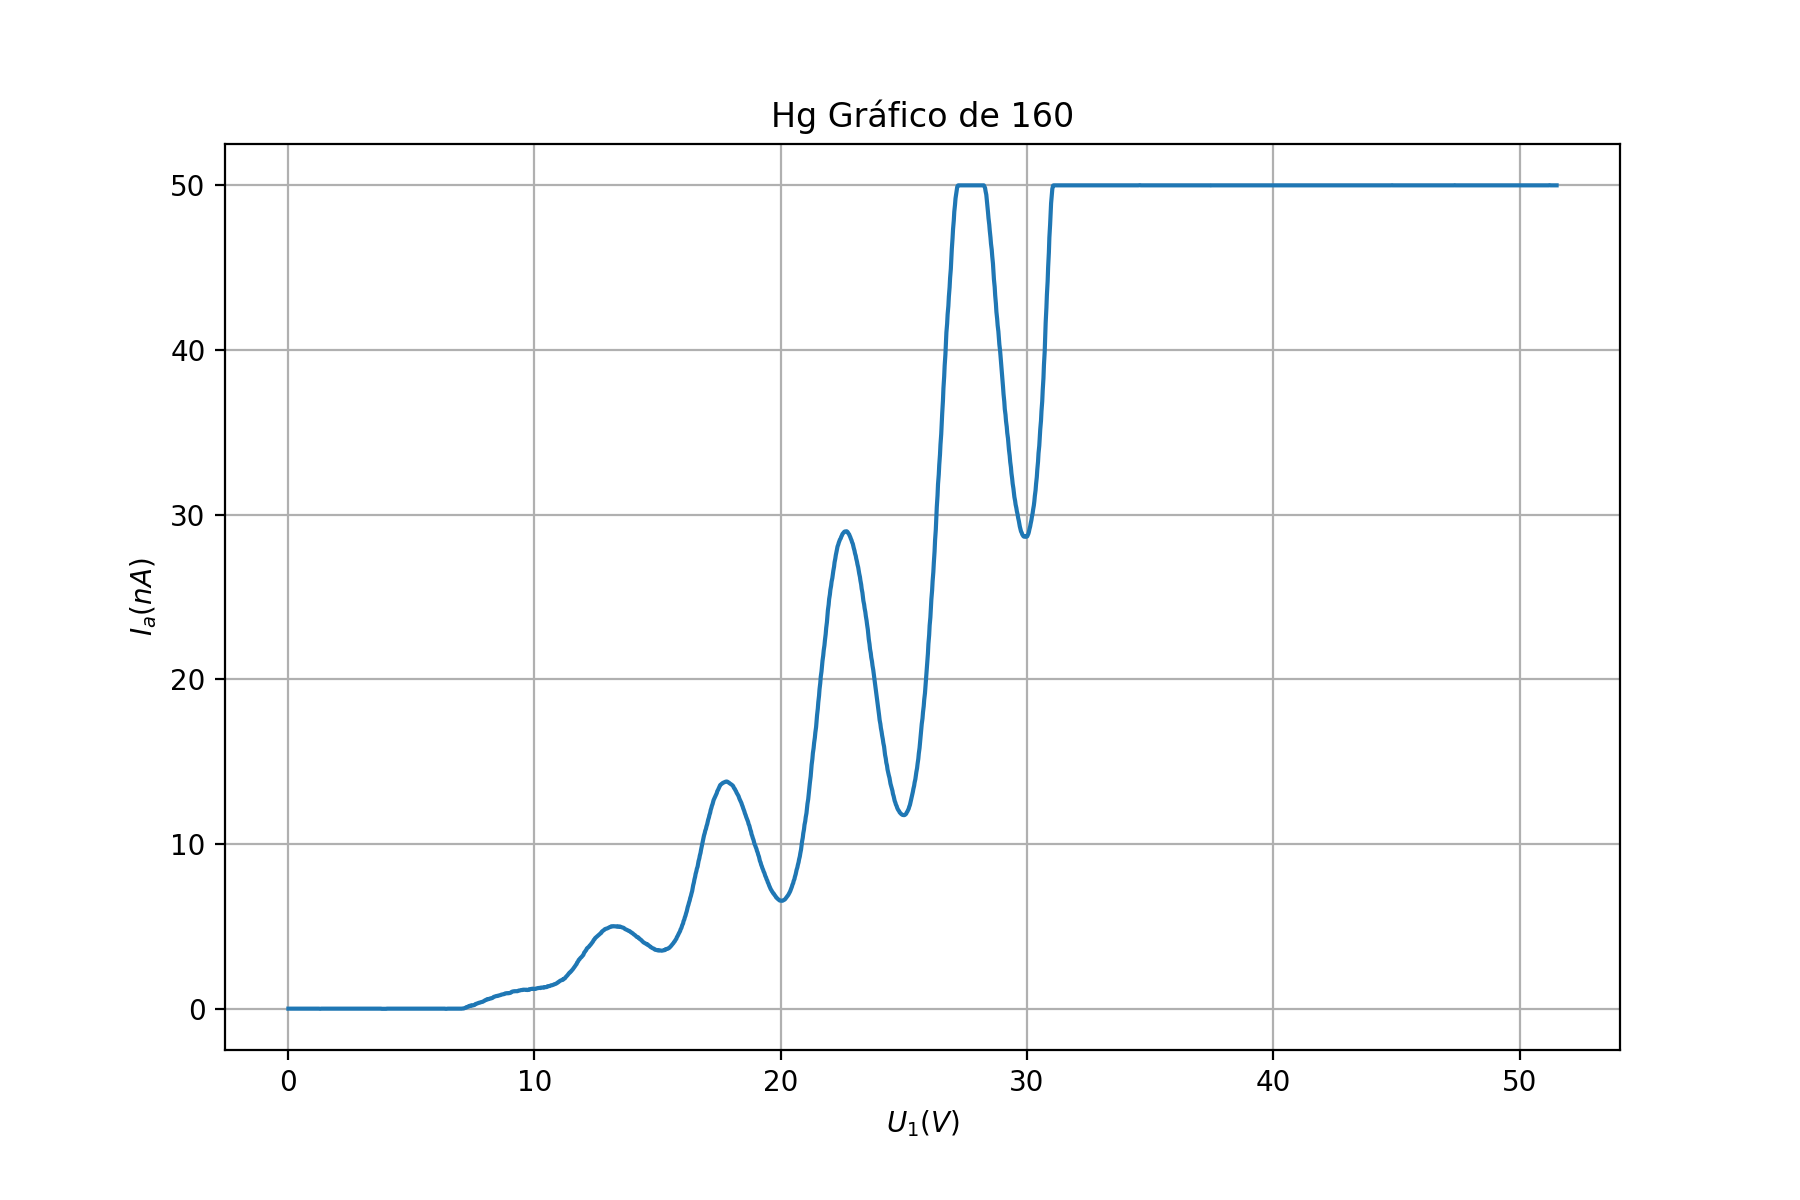
\includegraphics[max width=0.49\linewidth]{Hg Gráfico de 160}
\caption{Gráficas obtenidas para temperaturas de 145ºC, 150ºC, 155ºC y 160ºC respectivamente.}
\label{fig:tempsHg}
\end{center}
\end{figure}

\subsection{Dispositivo para el neón}

Para el caso del neón tenemos el dispositivo de la figura \ref{fig:FHNe}.

\begin{figure}[h!]
\begin{center}
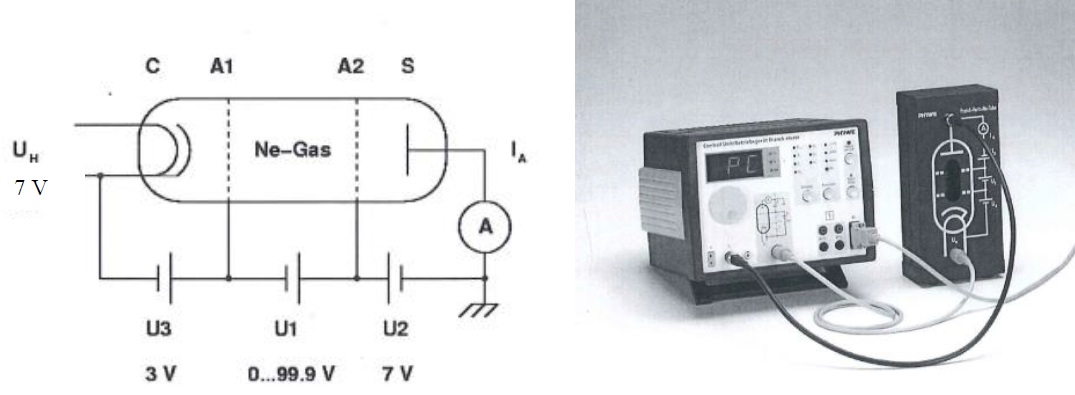
\includegraphics[max width=\linewidth]{FHNe}
\caption{Dispositivo de Frank-Hertz para el experimento con Neón.}
\label{fig:FHNe}
\end{center}
\end{figure}

El funcionamiento de este dispositivo es en principio similar al caso del mercurio, pero ligeramente distinto. Los elementos son los siguientes:

\begin{enumerate}
\item \textbf{C - Cátodo emisor de termoelectrones:} el funcionamiento es idéntico al ya explicado anteriormente. En este caso la tensión de calentamiento, $U_H$, se fija en 7V.
\item \textbf{A1 - Ánodo en forma de rejilla:} está cerca del cátodo C. Se aplica una diferencia entre C y A1, que llamamos $U_3$ que dirige los termoelectrones desde C hasta A1.
\item \textbf{A2 - Ánodo en forma de rejilla:} esta es la que se encarga de aplicar el potencial de aceleración $U_1$, que en este caso será variable desde 0 hasta 99.9V.
\item \textbf{S - Electrodo colector:} idénticamente al caso del mercurio, se aplica el voltaje $U_2$  y se mide la corriente recogida.
\end{enumerate}

El análisis que hacemos para el neón es idéntico al del mercurio. Realizaremos la curva $(U_1, I_A)$ y obtenemos el valor de la energía de excitación de la ecuación (\ref{eq:Ea}). Fuimos haciendo variar los parámetros del dispositivo, pero al final los mejores parámetros son los de la gráfica (\ref{fig:medNe}).

\begin{figure}[h!]
\begin{center}
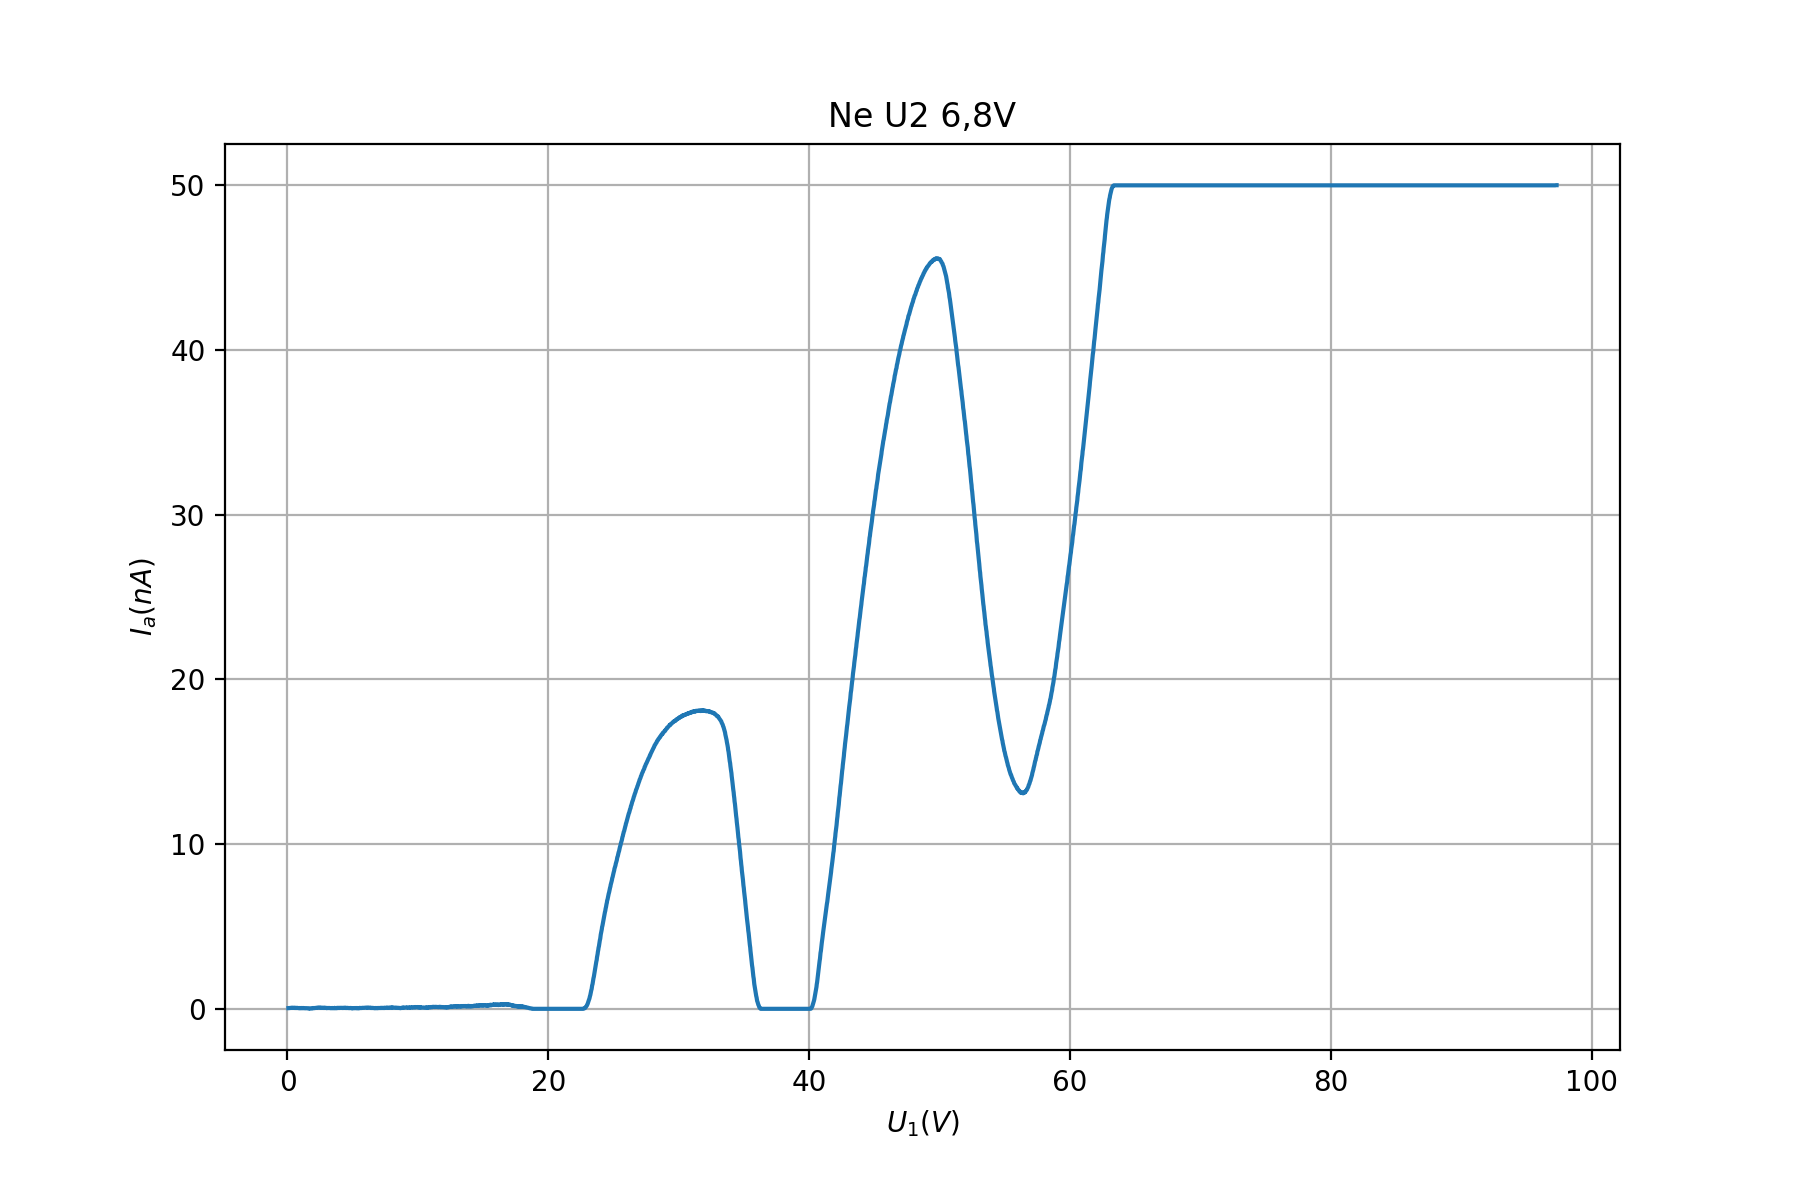
\includegraphics[max width=0.49\linewidth]{Ne U2 6,8V}
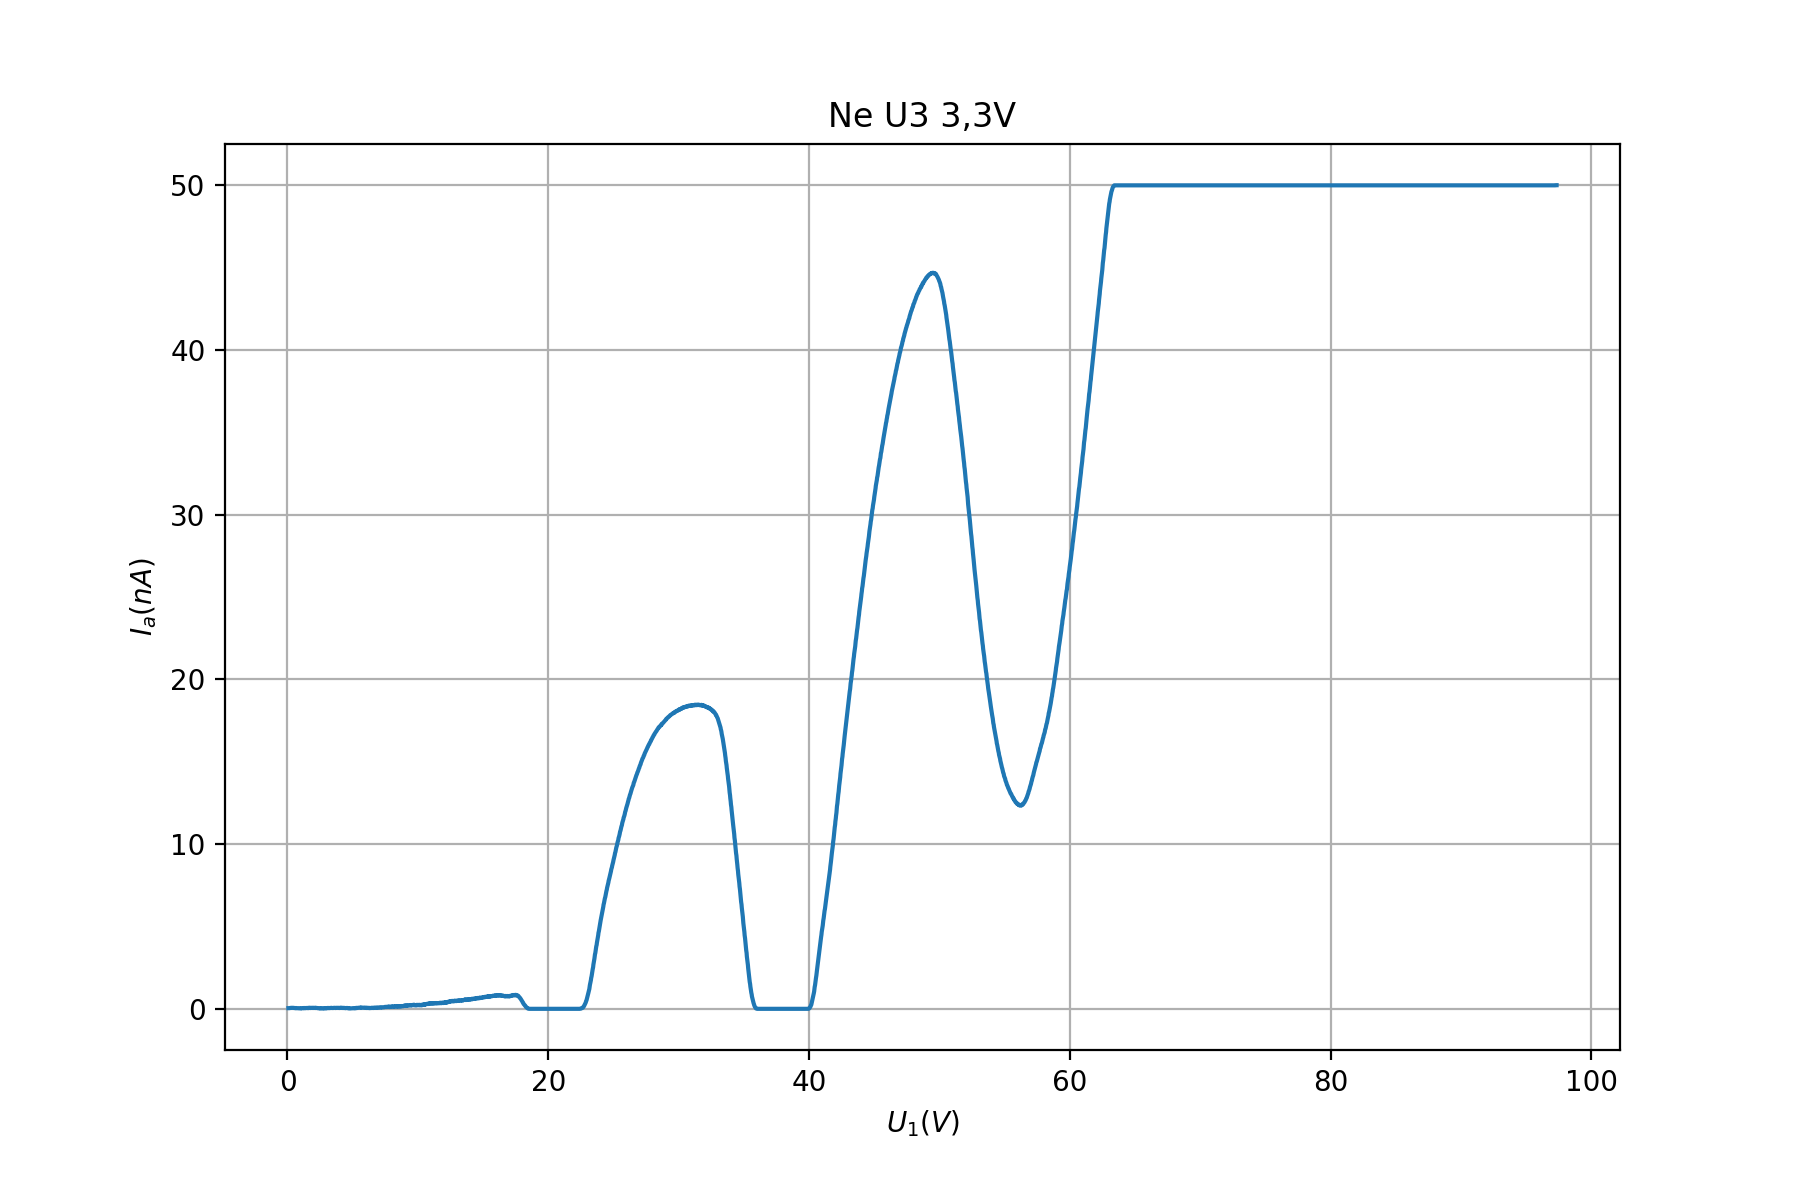
\includegraphics[max width=0.49\linewidth]{Ne U3 3,3V}
\caption{Las mejores gráficas obtenidas en la realización del experimento del neón. La primera tiene los parámetros estándar excepto que $U_2 = 6,8V$ mientras que la segunda utiliza los parámetros estándar poniendo $U_3 = 3,3V$.}
\label{fig:medNe}
\end{center}
\end{figure}

\section{Análisis de los datos}

Una vez hemos obtenido los datos que aparecen en la sección anterior, es hora de analizarlos. Para ello nos centraremos en la ecuación (\ref{eq:Ea}). Hay varias formas de obtener la energía de excitación.

Por un lado, podríamos considerar cada mínimo y hacer el cálculo con la energía de cada mínimo. Pero quizás es más interesante utilizar un ajuste lineal. Si representamos la curva $(n, U_{1, min})$ y ajustamos una recta a esta curva, debido a la ecuación (\ref{eq:Ea}) deberíamos obtener como pendiente la energía de activación.

También haremos un análisis siguiendo el artículo de R. Rubenza, para lo cual fuimos variando la temperatura. Esto es lo que se ve en la figura (\ref{fig:tempsHg}) que tendremos que tratar siguiendo la siguiente expresión. \cite{Rubenza}

\begin{equation}
\Delta U_{1, mín} = \left( 1 + \frac{l}{L}(2n - 1) \right) V_a
\end{equation}

\subsection{Energía de excitación del mercurio}

Realicemos un ajuste lineal para las gráficas de la figura (\ref{fig:medHg}). Se obtendrán las rectas que aparecen en la figura (\ref{fig:recHg}).

\begin{figure}[h!]
\begin{center}
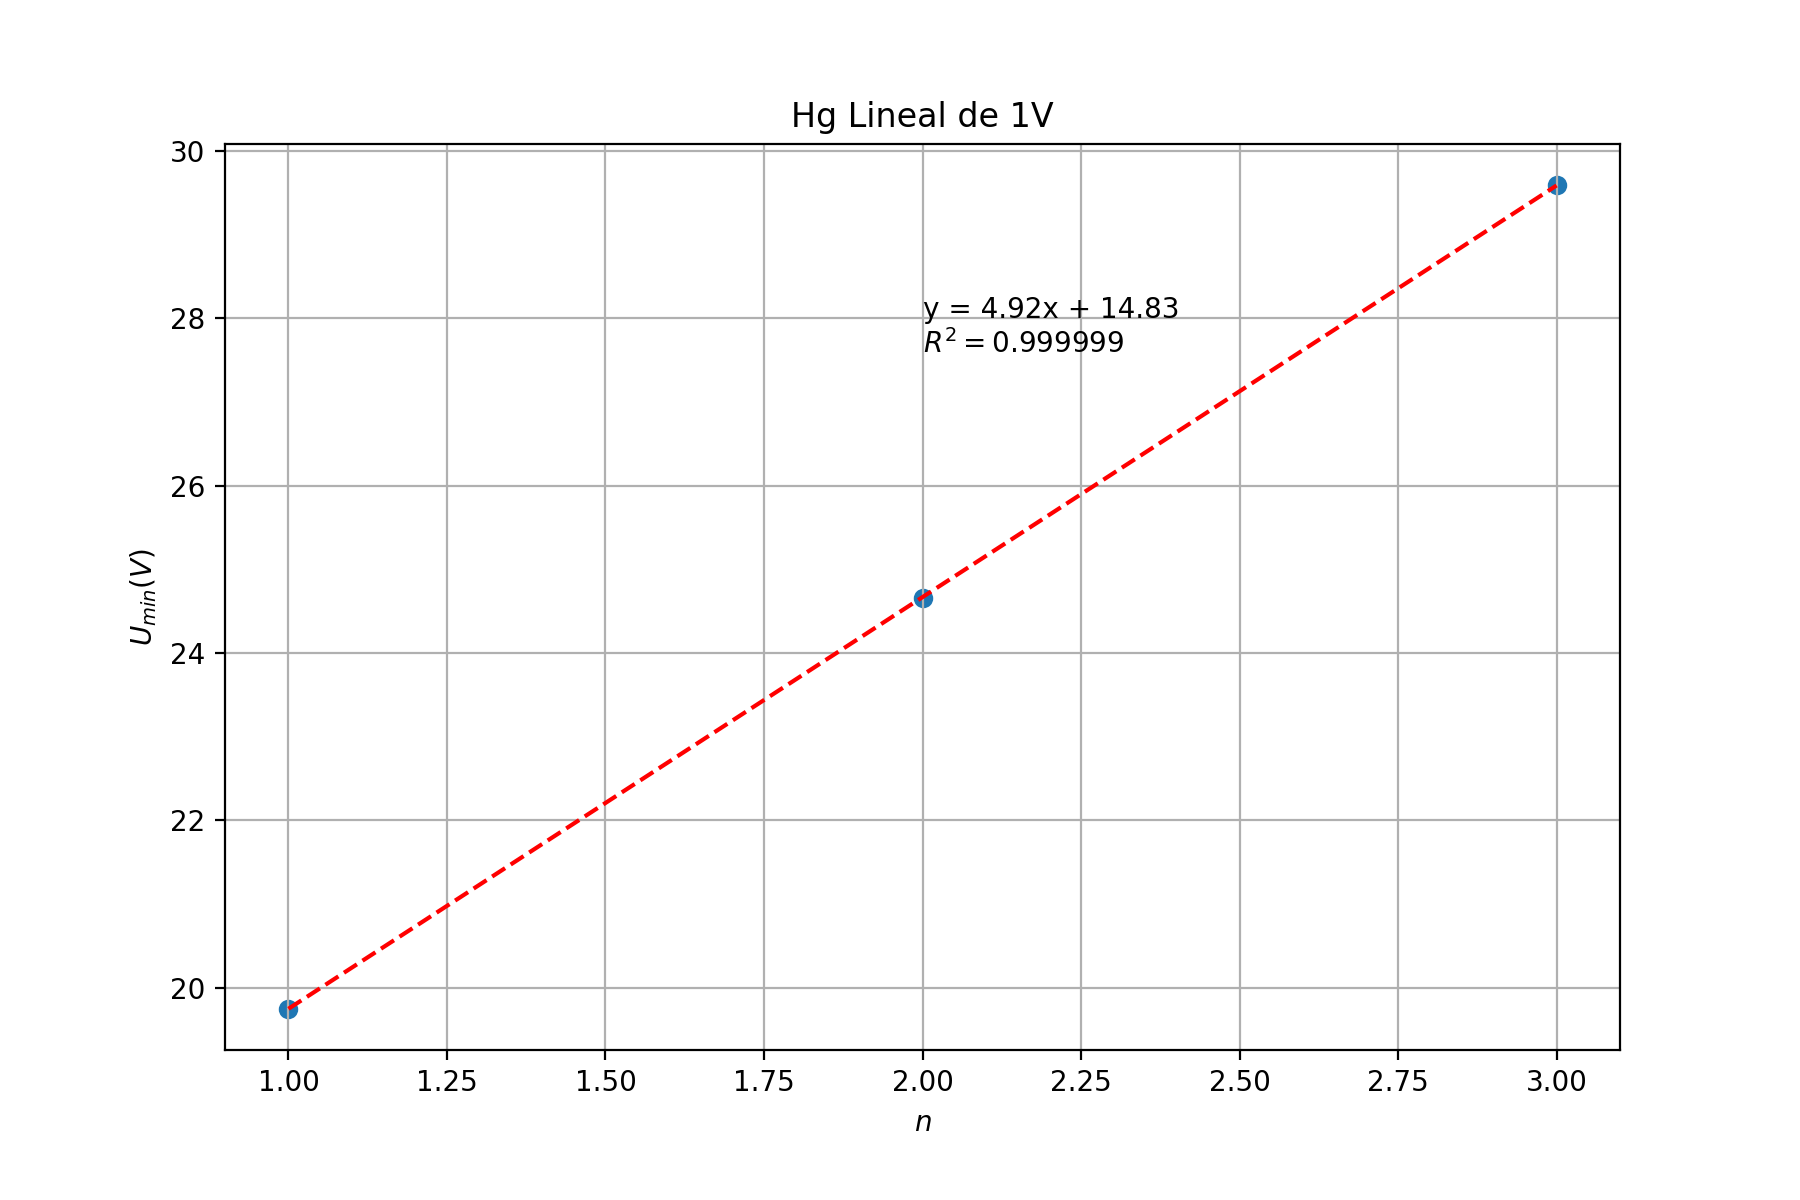
\includegraphics[max width=0.32\linewidth]{Hg Lineal de 1V}
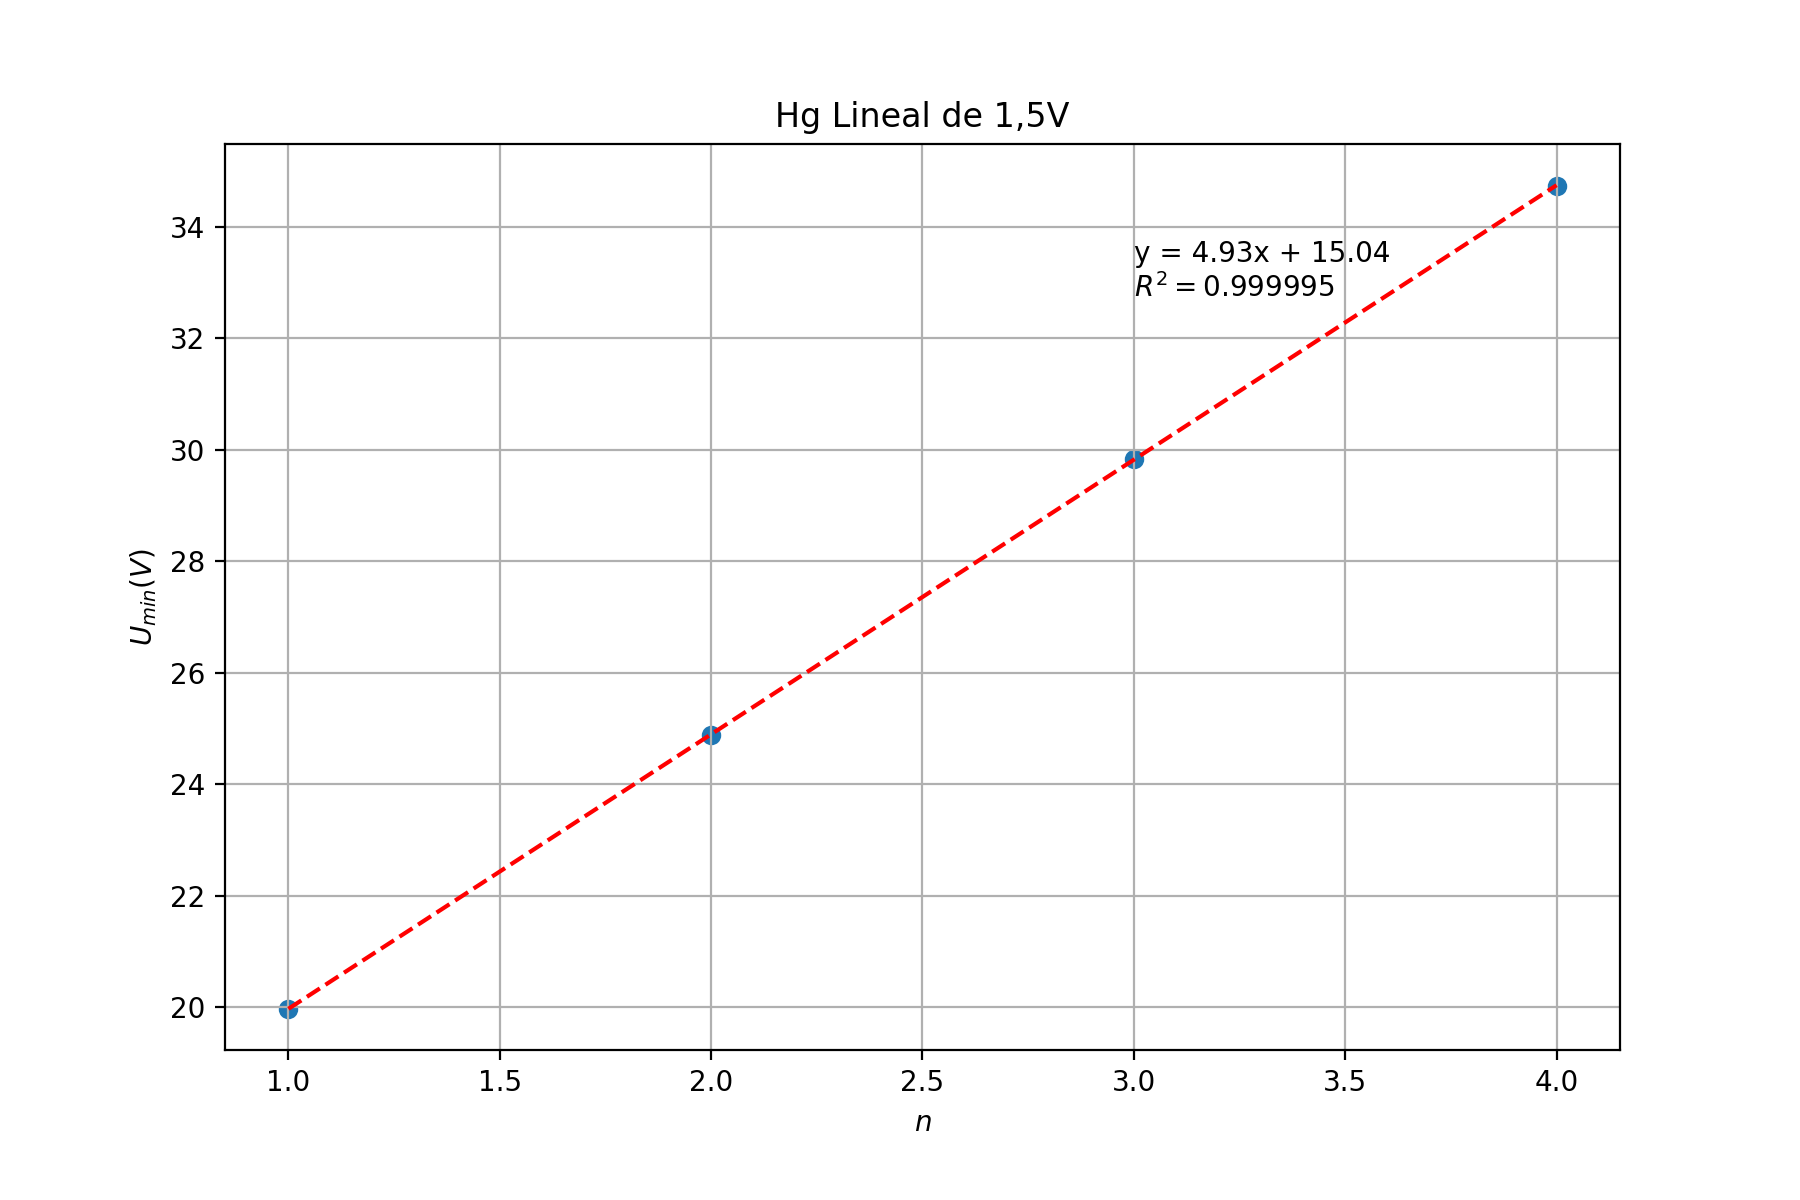
\includegraphics[max width=0.32\linewidth]{Hg Lineal de 1,5V}
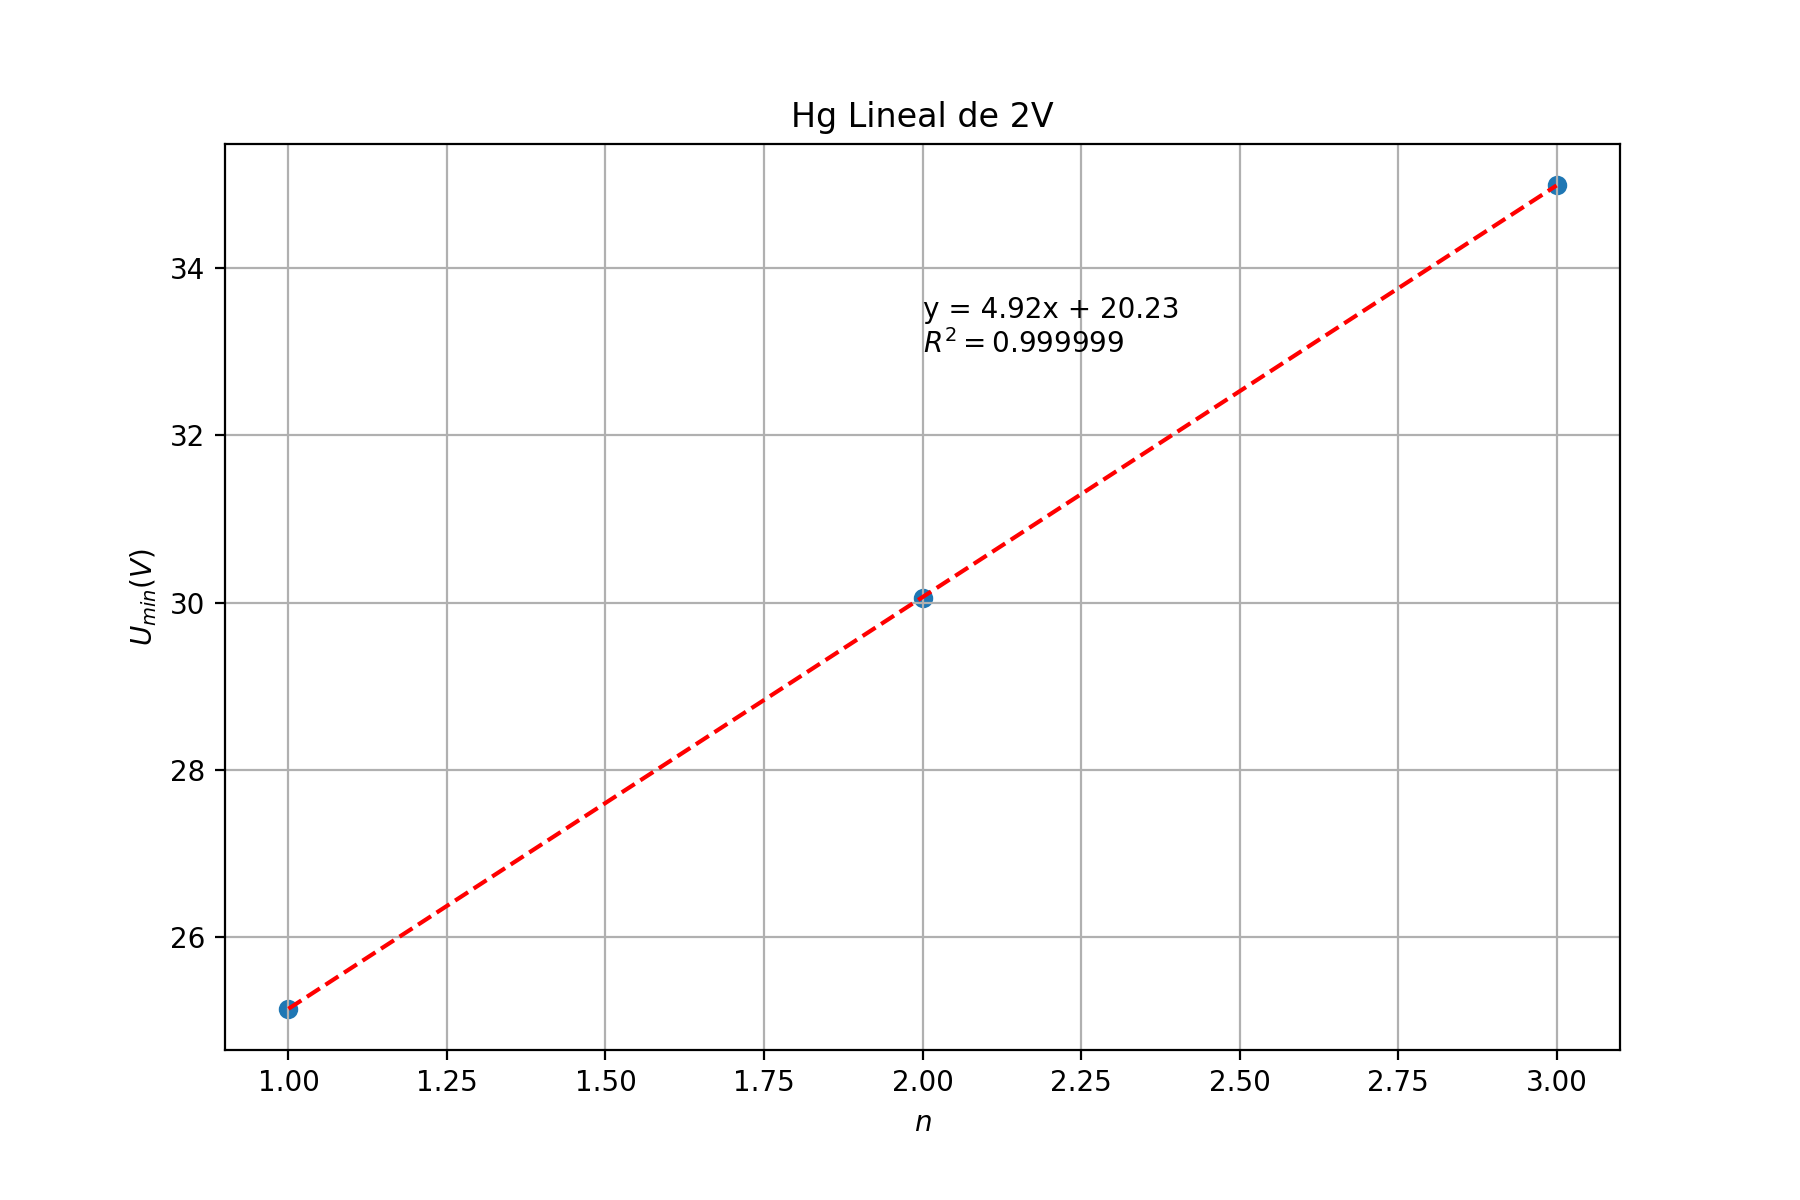
\includegraphics[max width=0.32\linewidth]{Hg Lineal de 2V}
\caption{Gráficas del ajuste lineal para el mercurio con potenciales de aceleración de 1V, 1,5V y 2V respectivamente. Los parámetros de la primera recta son $a = 4,920 \pm 0,005$, $b = 14,83 \pm 0,01$ y $R^2 = 0,9999986$. Los parámetros de la segunda recta son $a = 4,927 \pm 0,008$, $b = 15,04 \pm 0,02$ y $R^2 = 0,999994$. Los parámetros de la tercera recta son $a = 4,920 \pm 0,006$, $b = 20,23 \pm 0,01$ y $R^2 = 0,9999986$.}
\label{fig:recHg}
\end{center}
\end{figure}

Utilizando estos datos y con los dos procedimientos mencionados en la sección anterior, podemos encontrar valores de la energía de excitación. En la siguiente tabla se observan los resultados.

\begin{center}
\begin{tabular}{|c|c|c|c|}
\hline
$U_2 (V)$ & $1V$ & $1.5V$ & $2V$ \\ \hline \hline
$\Delta E$ (media) & $4.92 \pm 0.01 eV$ & $4.92 \pm 0.03 eV$ & $4.92 \pm 0.01 eV$ \\
$\Delta E$ (recta) & $4.920 \pm 0.006 eV$ & $4.927 \pm 0.008 eV$ & $4.920 \pm 0.006 eV$ \\ \hline
\end{tabular}
\captionof{table}{Tabla de las diferentes medidas para las energías de excitación.}
\end{center}

Podemos tomar una media ponderada de dichas medidas para cada valor de $U_2$ ya que la energía de activación será independiente, lo que nos da dos resultados con este método de hacer el experimento:

$$
\begin{array}{cc}
E_{a, media} = 4.92 \pm 0.03 eV & E_{a, recta} = 4,921 \pm 0,008 eV
\end{array}
$$

Y ya que tenemos los datos variando la temperatura también realizamos el mismo análisis para dichos datos. Las rectas de ajustes se observan en la figura (\ref{fig:rectTemp}).

\begin{figure}[h!]
\begin{center}
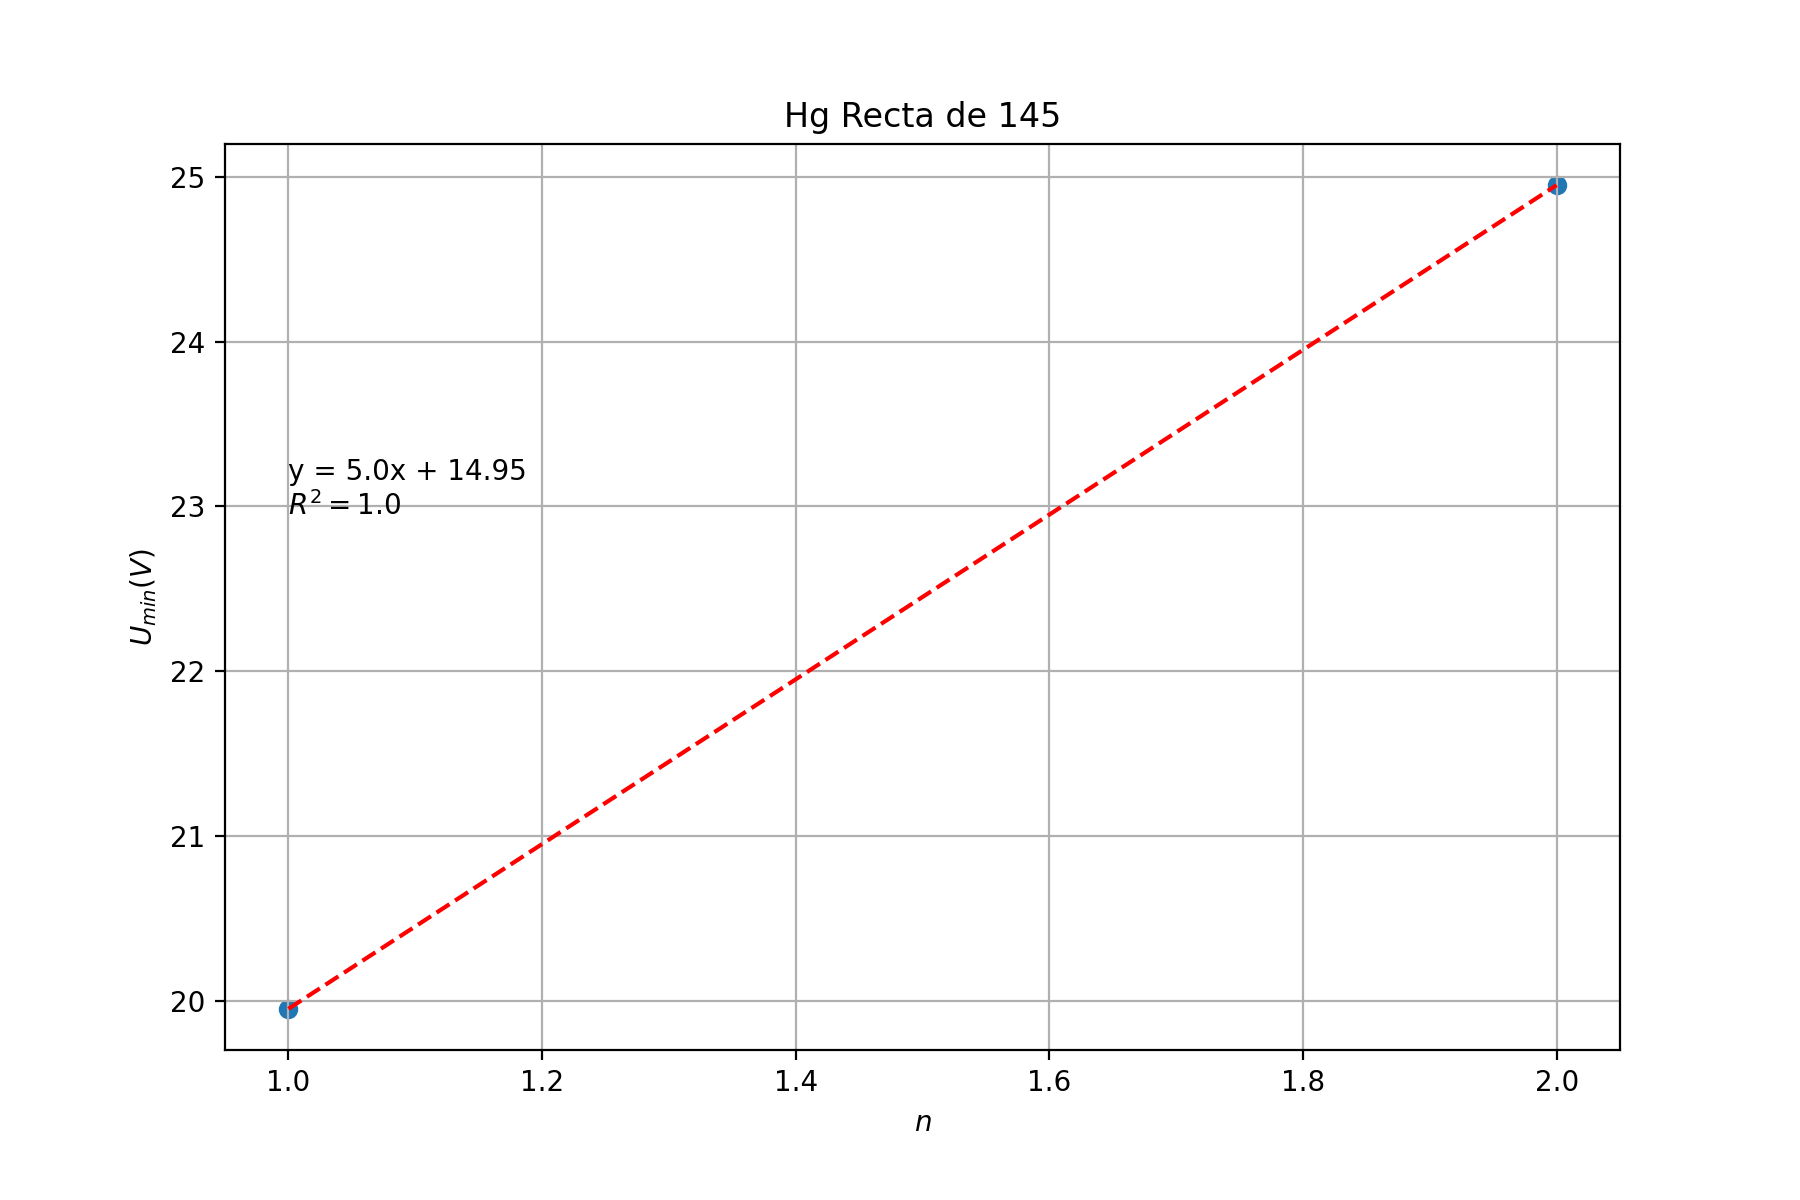
\includegraphics[max width=0.49\linewidth]{Hg Recta de 145}
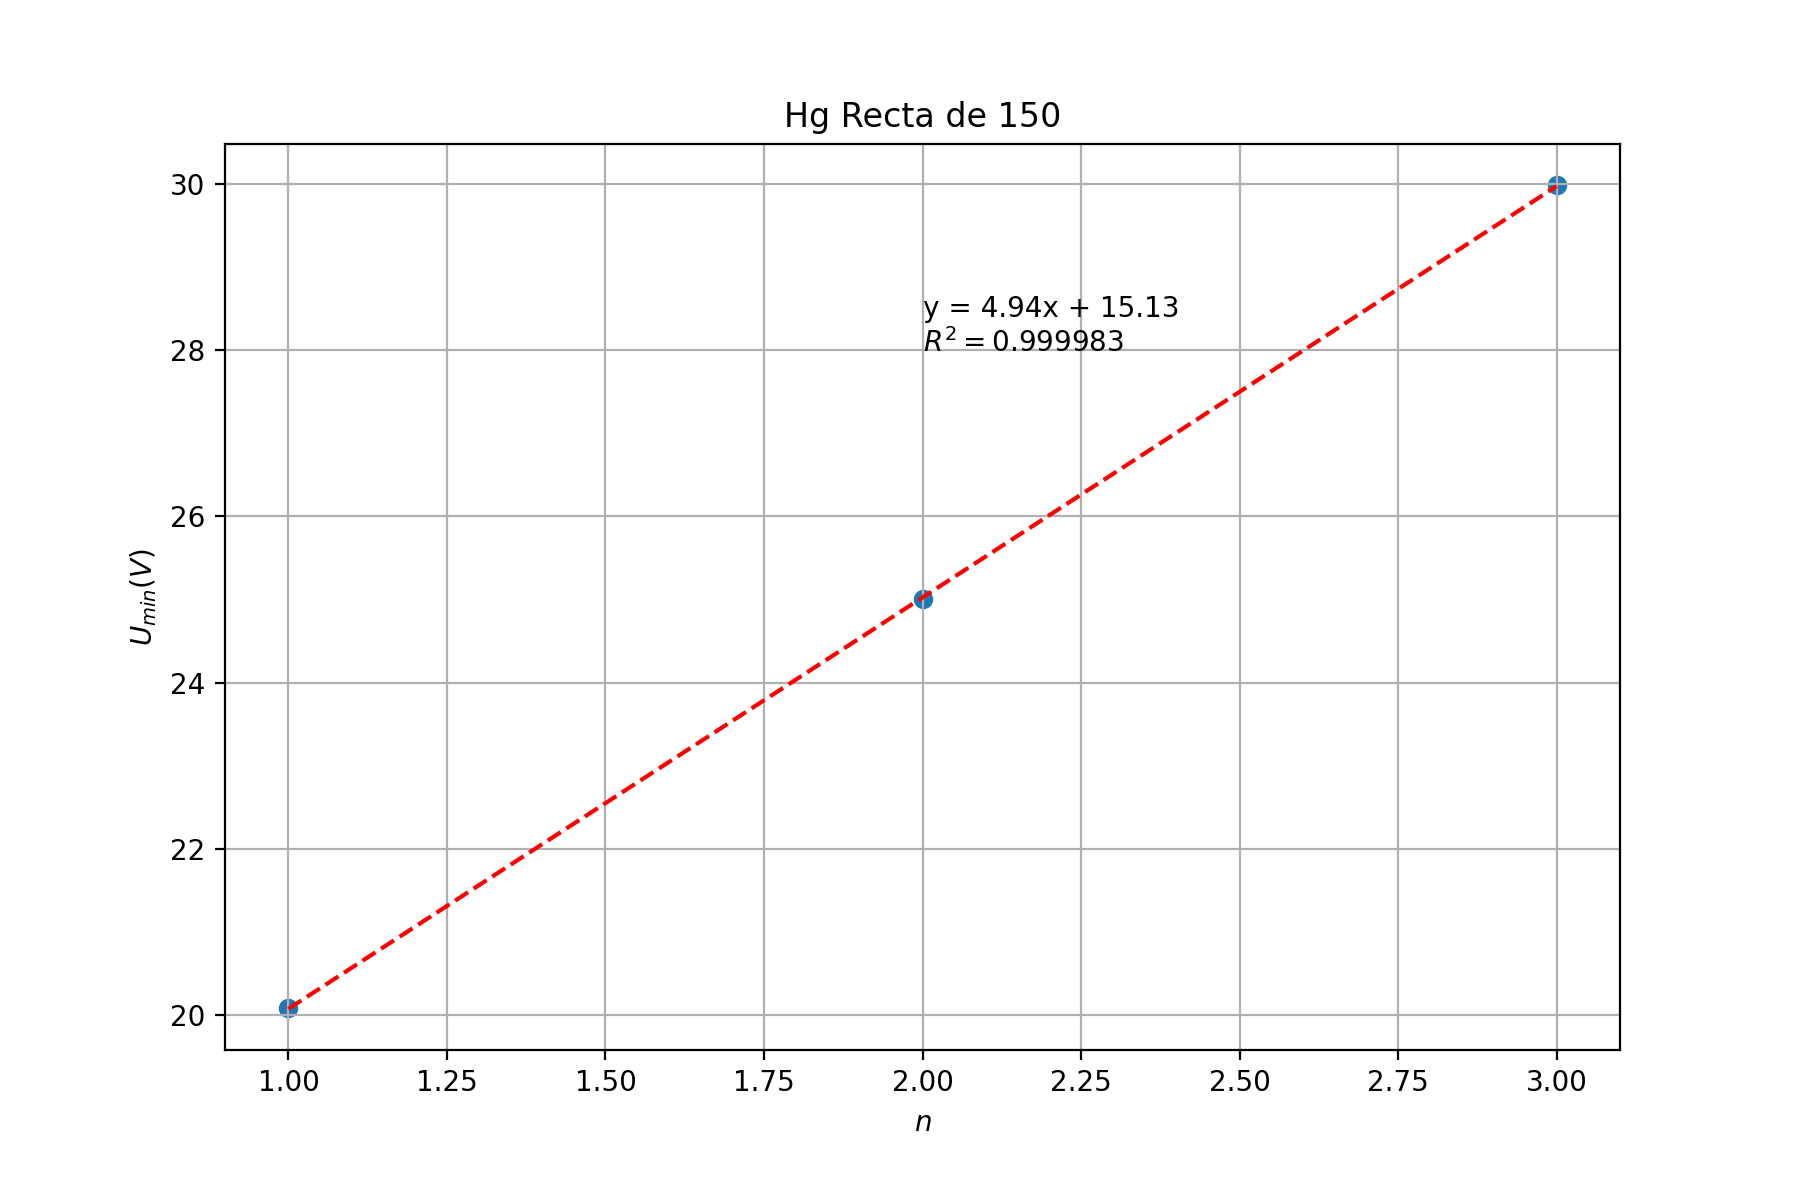
\includegraphics[max width=0.49\linewidth]{Hg Recta de 150}
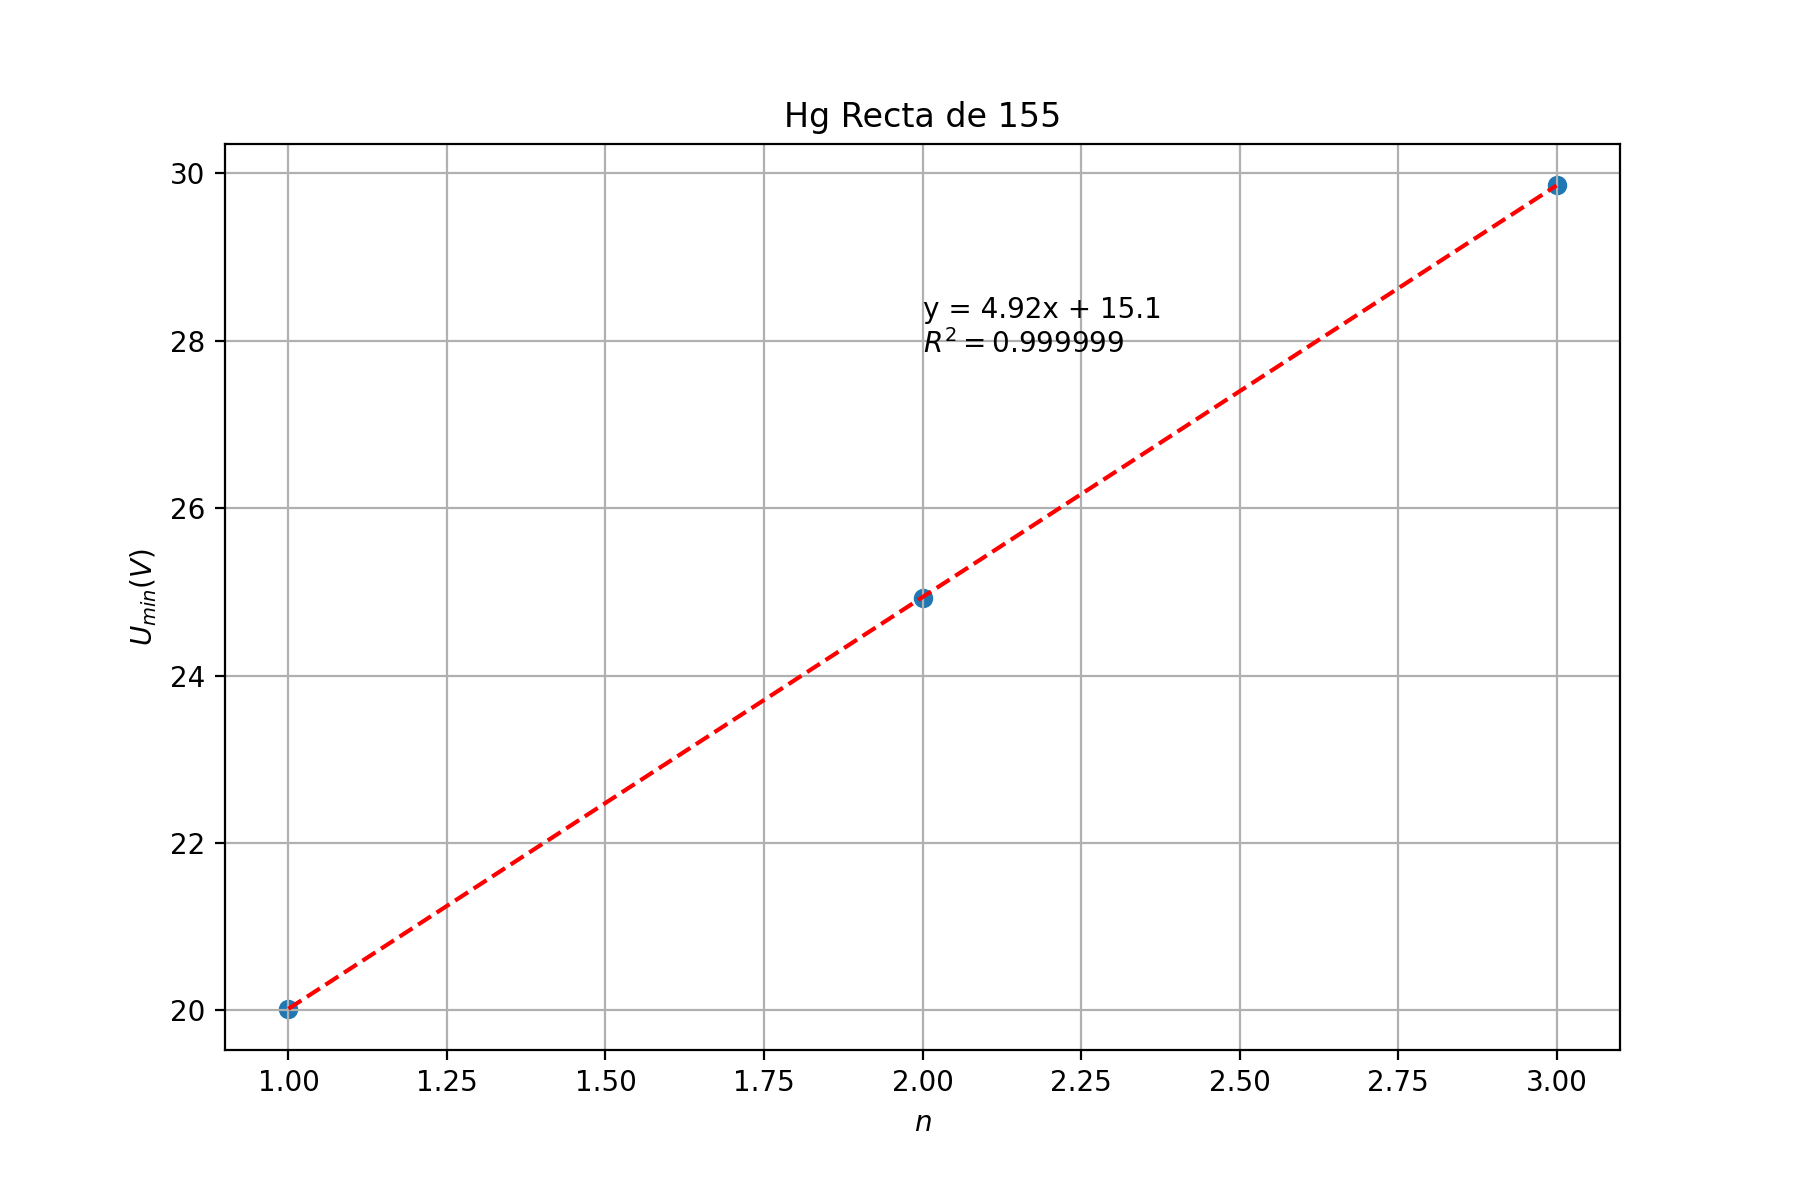
\includegraphics[max width=0.49\linewidth]{Hg Recta de 155}
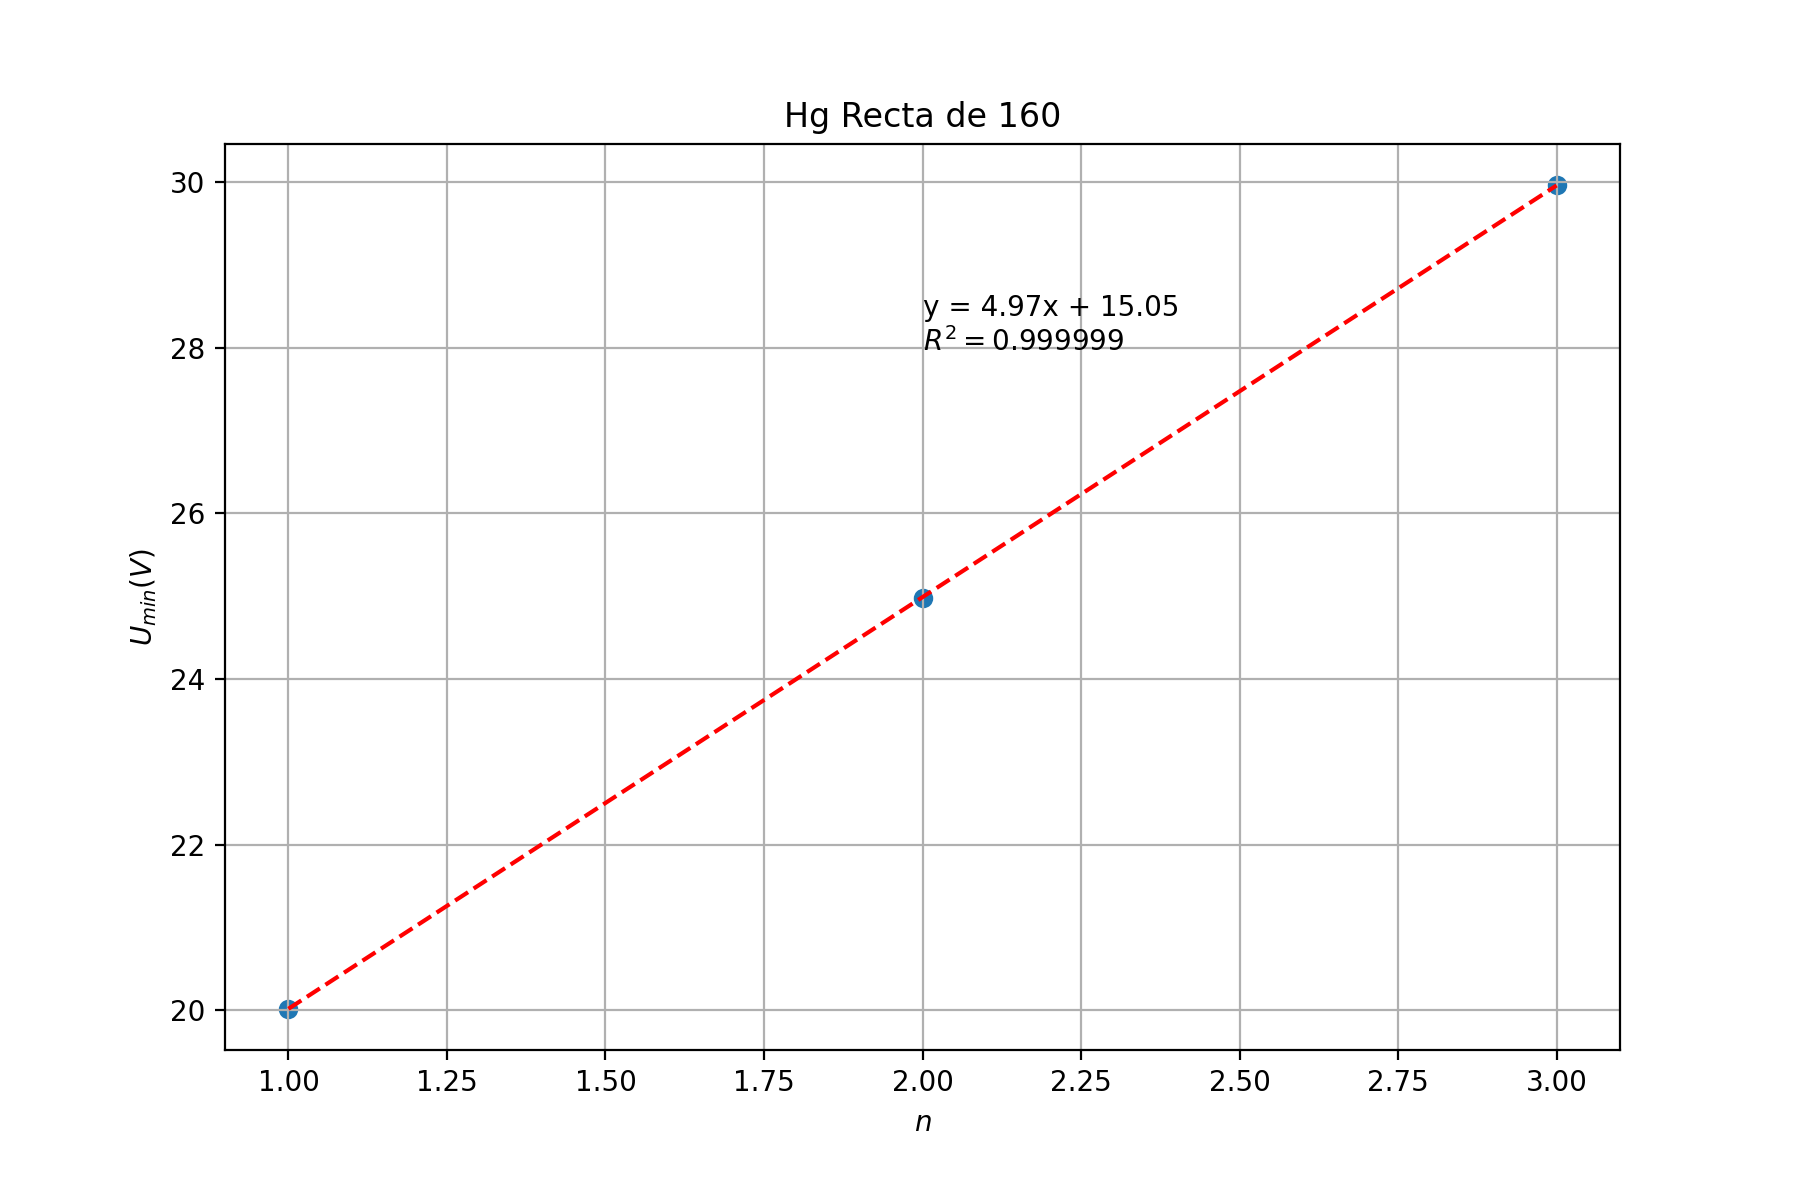
\includegraphics[max width=0.49\linewidth]{Hg Recta de 160}
\caption{Ajustes lineales al ir variando la temperatura. En la primera gráfica sólo conseguimos encontrar dos mínimos y no hay ajuste a hacer. En la segunda $a = 4.94 \pm 0.02$, $b = 15.13 \pm 0.04$ y $R^2 = 0.99998$. Para la tercera $a = 4.920 \pm 0.006$, $b = 14.10 \pm 0.01$ y $R^2 = 0.9999986$. Para la última $a = 4.970 \pm 0.006$, $b = 15.05 \pm 0.01$ y $R^2 = 0.9999987$}
\label{fig:rectTemp}
\end{center}
\end{figure}

En este caso, las medidas que obtenemos de la energía de excitación en cada gráfica son las siguientes:

\begin{center}
\hspace*{-0.25cm}\begin{tabular}{|c|c|c|c|c|}
\hline
T (ºC) & 145 & 150 & 155 & 160 \\ \hline \hline
$\Delta E$ (media) & $5.0 \pm 0.1 eV$ & $4.95 \pm 0.04 eV$ & $4.92 \pm 0.01 eV$ & $4.97 \pm 0.01 eV$ \\
$\Delta E$ (recta) & - & $4.94 \pm 0.02 eV$ & $4.920 \pm 0.006 eV$ & $4.970 \pm 0.006 eV$ \\ \hline
\end{tabular}
\captionof{table}{Tabla de las diferentes medidas para las energías de excitación en función de las temperaturas de medida.}
\end{center}

Repitiendo el proceso de la media ponderada obtenemos que la energía de excitación en estos casos es:

$$
\begin{array}{cc}
E_{a, media} = 4.945 \pm 0.007 eV & E_{a, recta} = 4.945 \pm 0.004 eV
\end{array}
$$

\subsection{Energía de excitación del neón}

En este caso los máximos no están claros, pues se escapan de la capacidad de medida de nuestro dispositivo. Para realizar el análisis y obtener la energía de excitación habrá que utilizar el procedimiento de tomar medias. En este caso las medidas no saldrán tan bien pero sí que habrá una coincidencia con el valor de la bibliografía \cite{Neon}.

$$
\begin{array}{cc}
E_{a, 1} = 20 \pm 5 eV & E_{a, 2} = 20 \pm 1 eV
\end{array}
$$

Que haciendo la media ponderada nos queda que:

$$
E_a = 20 \pm 1 eV
$$

Mencionemos que no podemos realizar ajustes lineales pues sólo tenemos dos máximos lo que no nos permite hacer un ajuste correcto por mínimos cuadrados.

Utilizando la expresión (\ref{eq:lambda}) podemos obtener la longitud de onda a la que emite, que situamos en:

$$
\lambda = 590 \pm 90 nm
$$

\subsection{Recorrido libre medio}

Haremos un análisis según la referencia \cite{Rubenza}. En este caso, tenemos pocos mínimos identificados, por lo que haremos la representación de $(2n-1, \Delta U_{1, min})$ donde la pendiente será $\frac{l}{L} V_a$ y el valor de $V_a$ se puede obtener de la ordenada en el origen. Las gráficas que tenemos son las siguientes:

\begin{figure}[h!]
\begin{center}
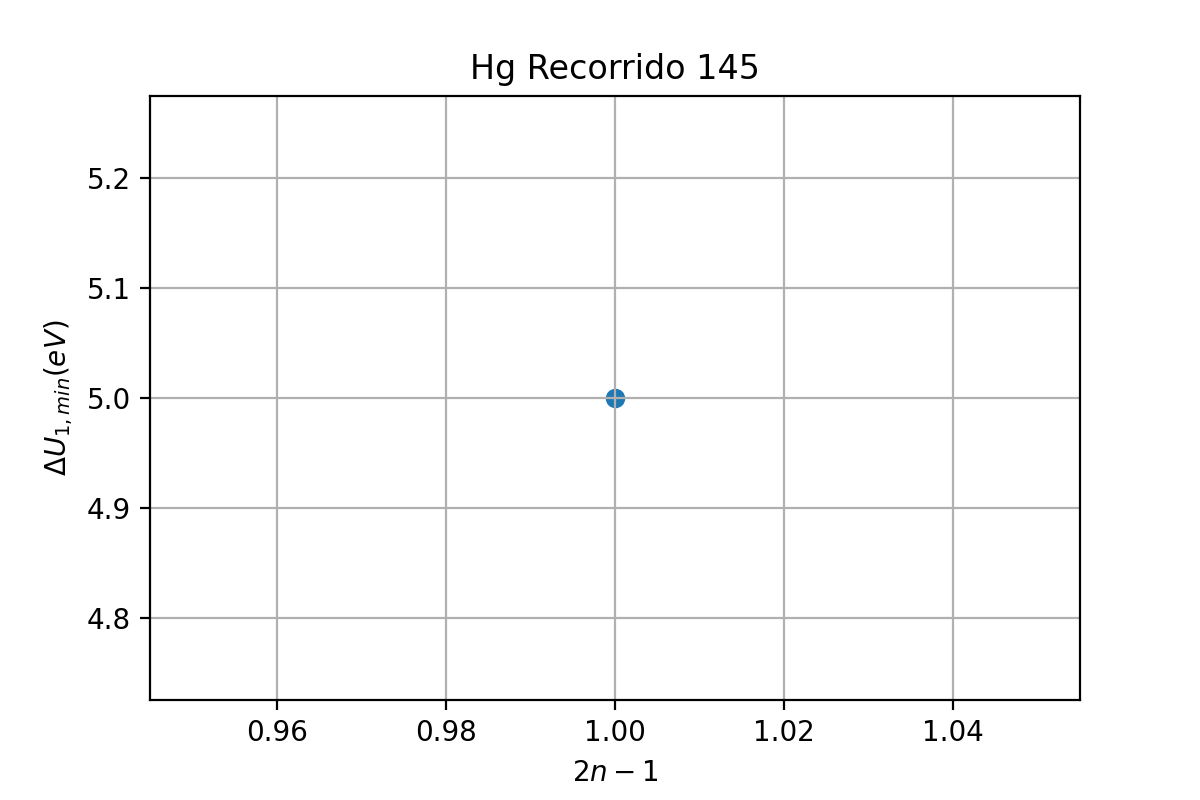
\includegraphics[max width=0.49\linewidth]{Hg Recorrido 145}
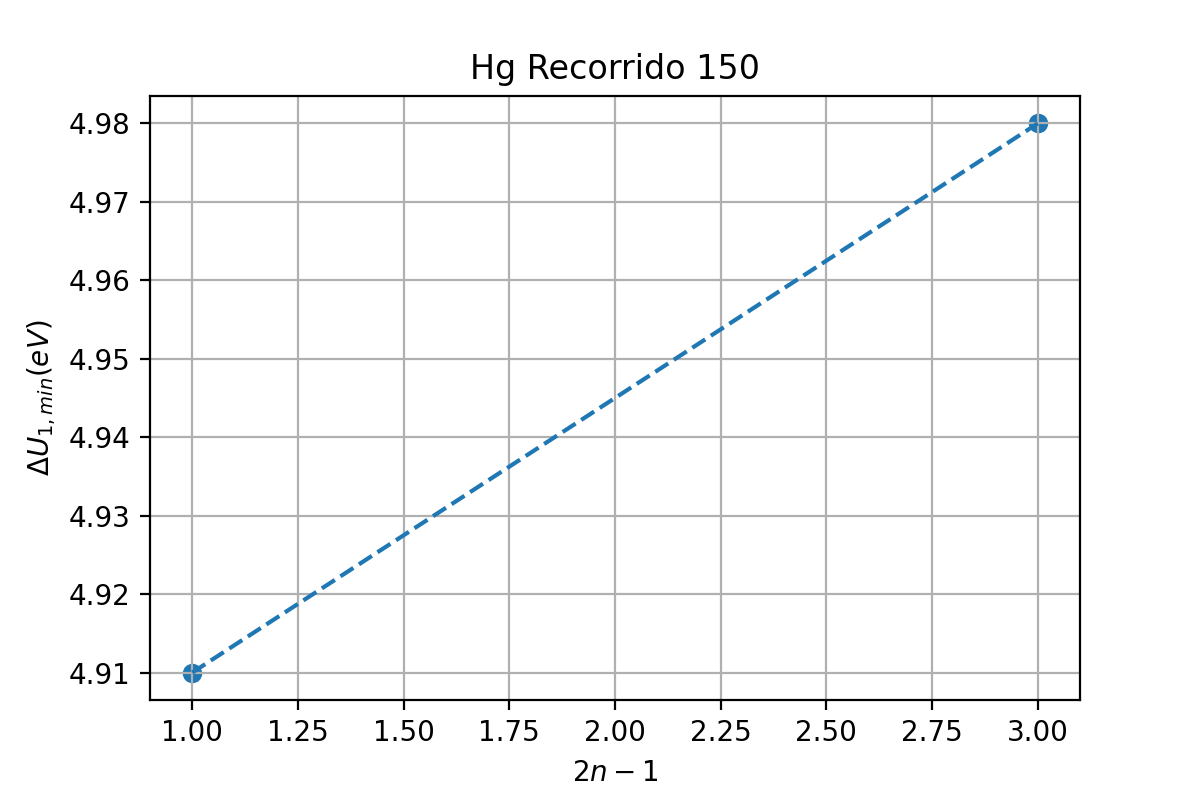
\includegraphics[max width=0.49\linewidth]{Hg Recorrido 150}
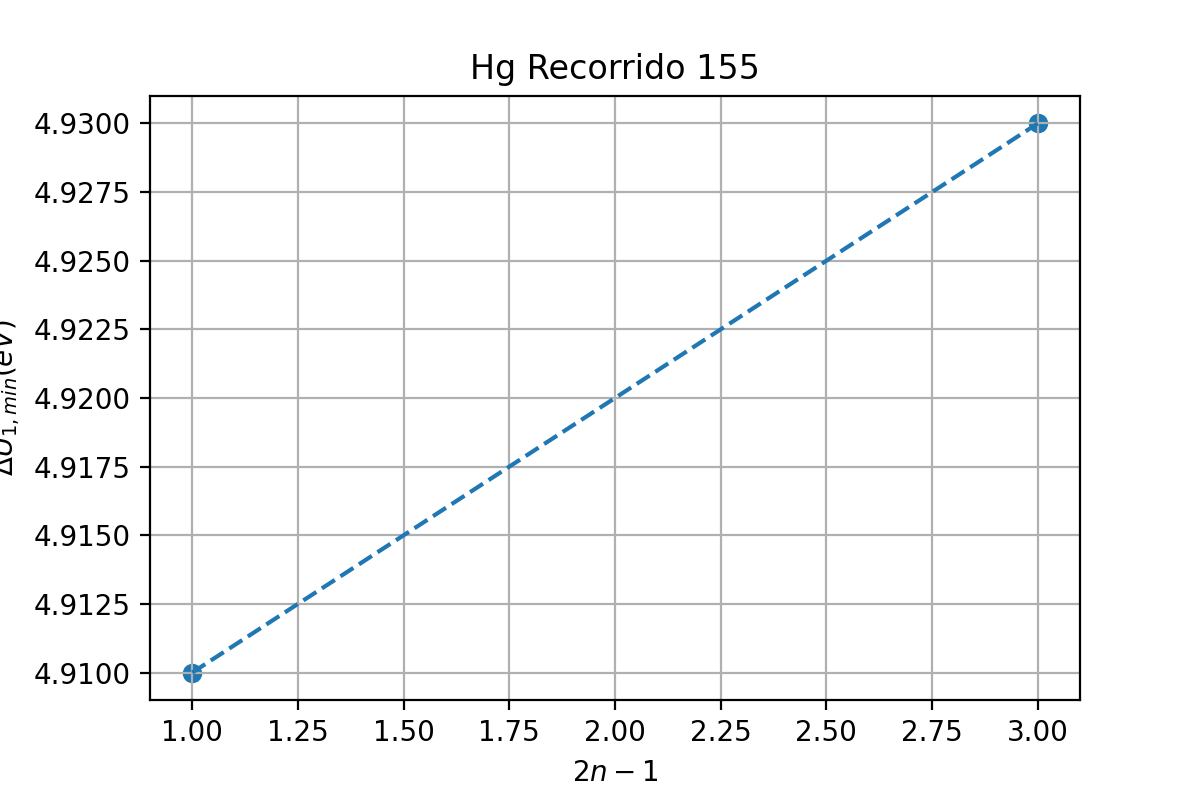
\includegraphics[max width=0.49\linewidth]{Hg Recorrido 155}
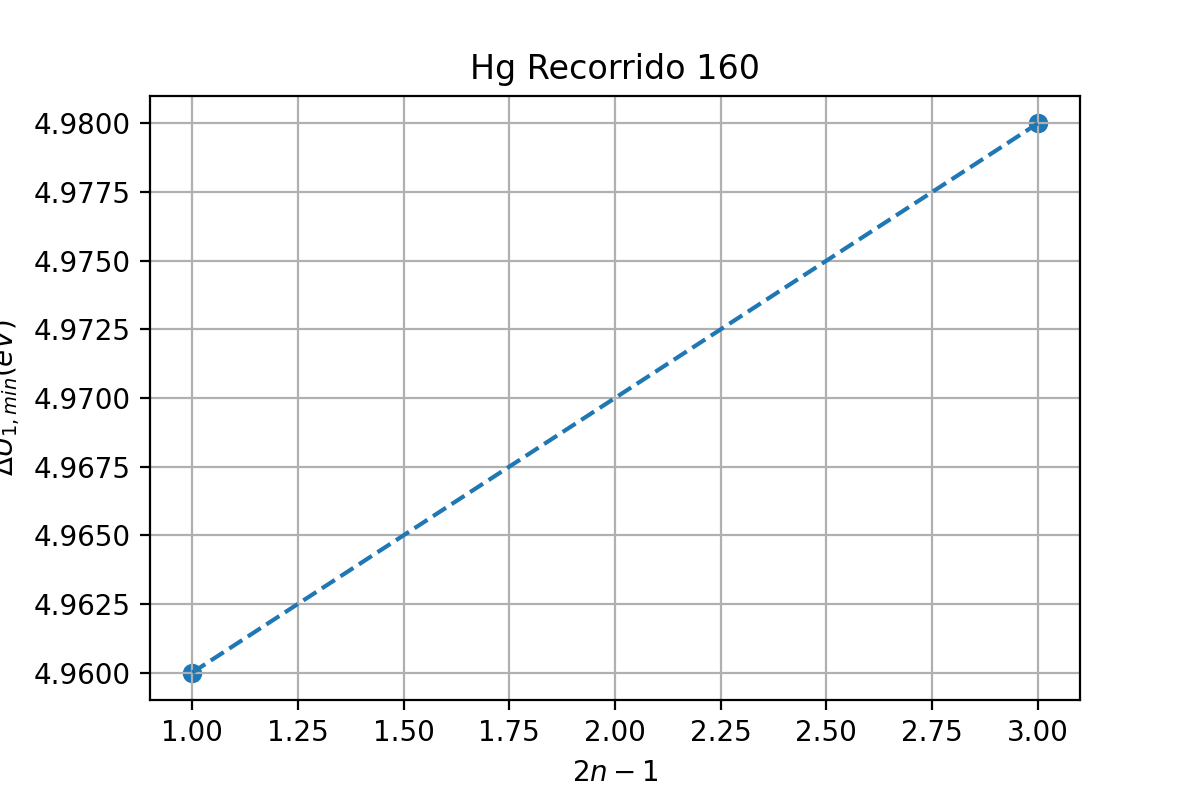
\includegraphics[max width=0.49\linewidth]{Hg Recorrido 160}
\caption{Ajustes para el recorrido libre medio, aunque en ninguna se obtienen más de dos puntos.}
\end{center}
\end{figure}

Claramente en el primer caso no hay nada que hacer. En el resto de casos vamos a representar el recorrido libre medio en función de L siendo esta la distancia entre el emisor de termoelectrones y la placa receptora.

Obtenemos que:

\begin{center}
\begin{tabular}{|c|c|c|c|c|}
\hline
T (ºC) & 145 & 150 & 155 & 160 \\ \hline \hline
l & - & 0.0072L & 0.002L & 0.002L \\ \hline
\end{tabular}
\captionof{table}{Tabla de las medidas del recorrido libre medio en términos de L, ya ajustados al valor de $V_a$.}
\end{center}

Discutiremos que efectos puede tener la falta de puntos sobre esta medida.

El artículo \cite{Rubenza} nos da también una forma de calcular la presión dentro del tubo aproximadamente.

\begin{equation}
P = 8,7 \times 10^{9 - \frac{3110}{T}}
\end{equation}

\section{Discusión de resultados}

Para el caso del mercurio hemos obtenido cuatro valores de la energía de excitación de dicho elemento. Estos cuatro valores concuerdan todos con los de la bibliografía. Ahora, cabe preguntarse, ¿podemos combinar dichos resultados?

Pues, podemos combinar los correspondientes a las rectas en ambos experimentos (variando $U_2$ y variando la temperatura) así como los correspondientes a las medias pues son datos que emergen de experimentos distintos.

Sin embargo, no podemos combinar las rectas y las medias, pues sería tener en cuenta dos veces datos que pertenecen al mismo experimento, con esto, tenemos dos valores de la energía de excitación en función de qué procedimiento sigamos para analizar los datos.

$$
\begin{array}{cc}
E_{a, media} = 4.944 \pm 0.007 eV & E_{a, recta} = 4.940 \pm 0.004 eV
\end{array}
$$

En este caso, los errores relativos de las medidas son 0.14\% y 0.08\% respectivamente, lo que las convierte en unas muy buenas medidas.

Para el caso del neón hemos obtenido que su energía de activación y la longitud de onda a la que emite es de:

$$
\begin{array}{cc}
E_a = 20 \pm 1 eV & \lambda = 590 \pm 90 nm
\end{array}
$$

Esta longitud de onda es consistente con el color que veíamos emitir al neón, coincide en error con el rango del anaranjado. La energía de excitación tiene un error relativo del 5\% que está al límite de lo aceptable.

Finalmente, en el caso del recorrido libre medio los resultados no son muy buenos debido a la falta de puntos. Además, tienen unos errores demasiado grandes cuando los cuantificamos, pero en general, si hacemos como en \cite{Rubenza} y tomamos $L = 1cm$ veremos que los valores coinciden dentro de error con los de este experimento, siendo que, por ejemplo, para 155ºC, $l \approx 72 \mu m$.

\section{Conclusiones}

Se concluye que los valores que se obtienen para las energías excitadas son válidos y coinciden con los valores de la bibliografía en error, siendo que se comprueba claramente la naturaleza cuantizada de la materia. También podemos observar la emisión por transición de electrones.

Por otro lado, el caso del recorrido libre medio no es muy satisfactorio puesto que faltan puntos y medidas. Habría que juguetear con los parámetros del dispositivo, o incluso usar otro dispositivo más sensible a intensidades menores, en cualquier caso, en el artículo de R. Rubenzahl \cite{Rubenza} se obtienen también unos errores muy grandes para el recorrido libre medio, lo que permite que nuestras medidas coincidan con dicho artículo.

Las posibles fuentes de error probablemente se deban al método de seleccionar los mínimos (o máximos) ya que lo hacíamos con el programa en sí de medida y en el proceso perdíamos algún punto por el camino.

En general, considero cumplido el objetivo del experimento. Se han obtenido las energías de los estados excitados del mercurio y del neón, con un error bastante bajo y se observa claramente la naturaleza cuántica de la materia.

\section{Anexo 1: fórmulas de error}

La fórmula del error cuando utilizamos la media para obtener los valores de la energía de excitación es:

$$
\frac{\Delta E_a}{e} = \frac{\Delta U_{1, min}}{n}
$$

Aunque no se utiliza mucho ya que por lo general, la desviación estándar de la media es mayor a este error.

Para la medida de la longitud de onda en el caso del neón usamos para calcular el error que:

$$
\Delta \lambda = \frac{hc}{E_a - E_{3s}} \Delta E_a
$$

\section{Anexo 2: el código}

Para la realización de esta práctica se ha desarrollado un código en Python que lee los datos del programa en formato .txt y los analiza siguiendo una serie de procedimientos, esto nos ha permitido analizar rápidamente los datos de cada experimento.

Dicho código en Python, así como el código en Latex para este informe, las imágenes en alta resolución y los datos exportados del programa de medida, se pueden encontrar en un repositorio de GitHub siguiendo este enlace:

\section{Anexo 3: datos descartados}

En el caso del neón, se incluyen aquí las gráficas de los experimentos descartados:

\begin{figure}[h!]
\begin{center}
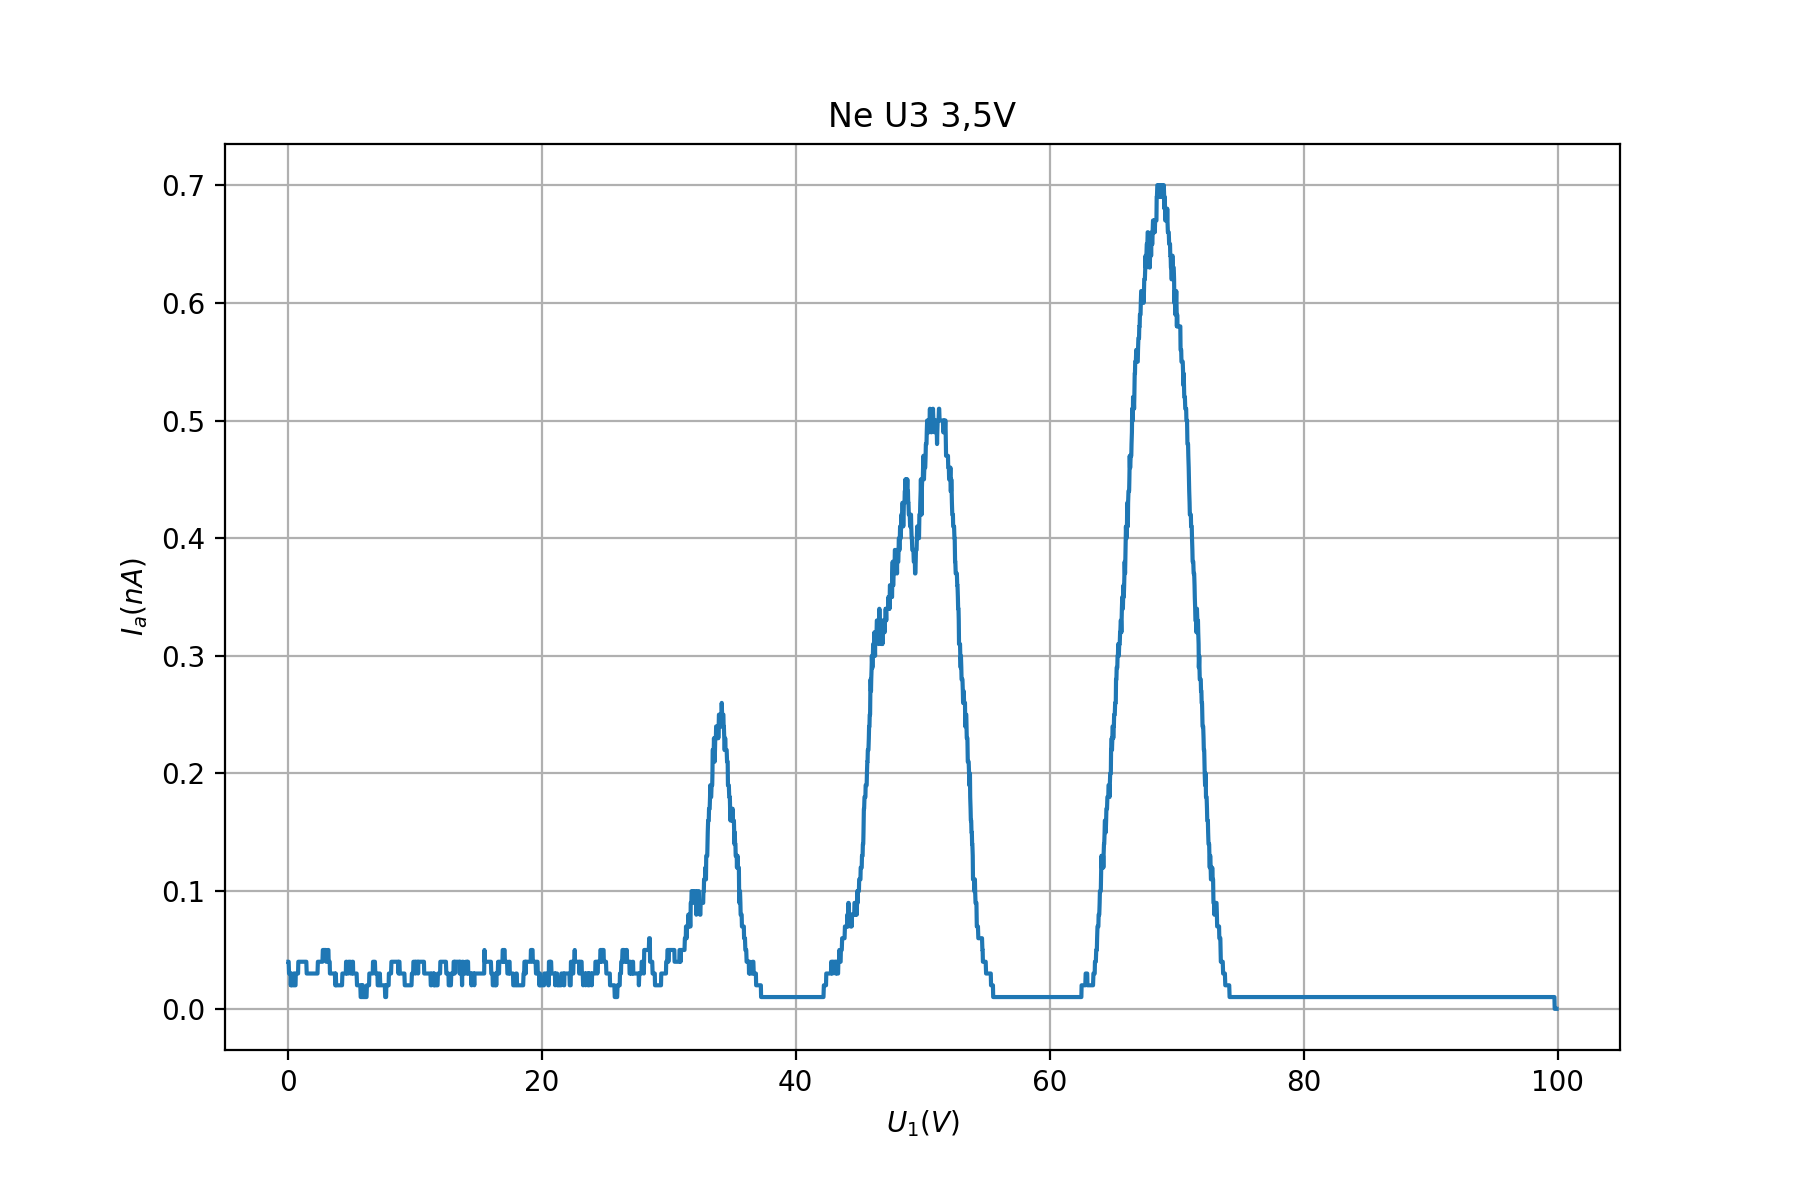
\includegraphics[max width=0.32\linewidth]{Ne U3 3,5V}
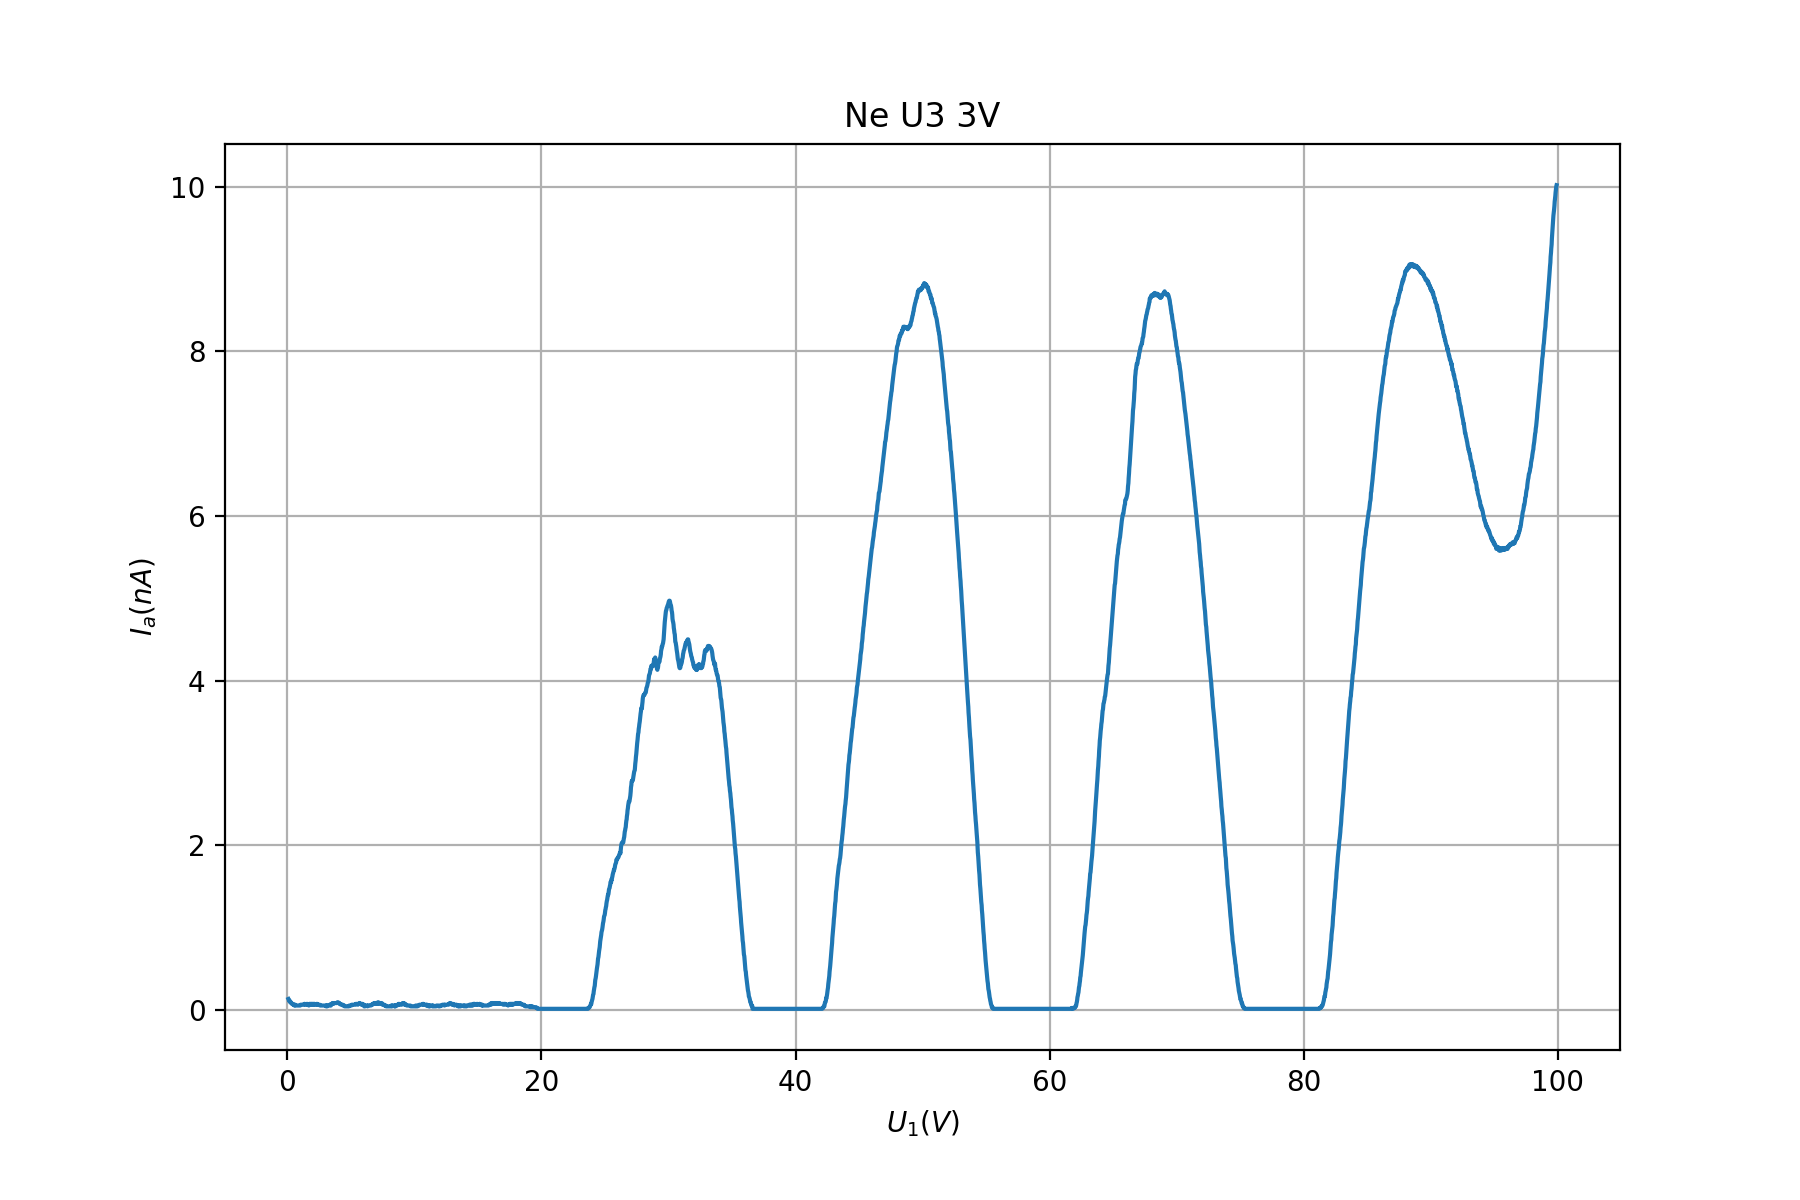
\includegraphics[max width=0.32\linewidth]{Ne U3 3V}
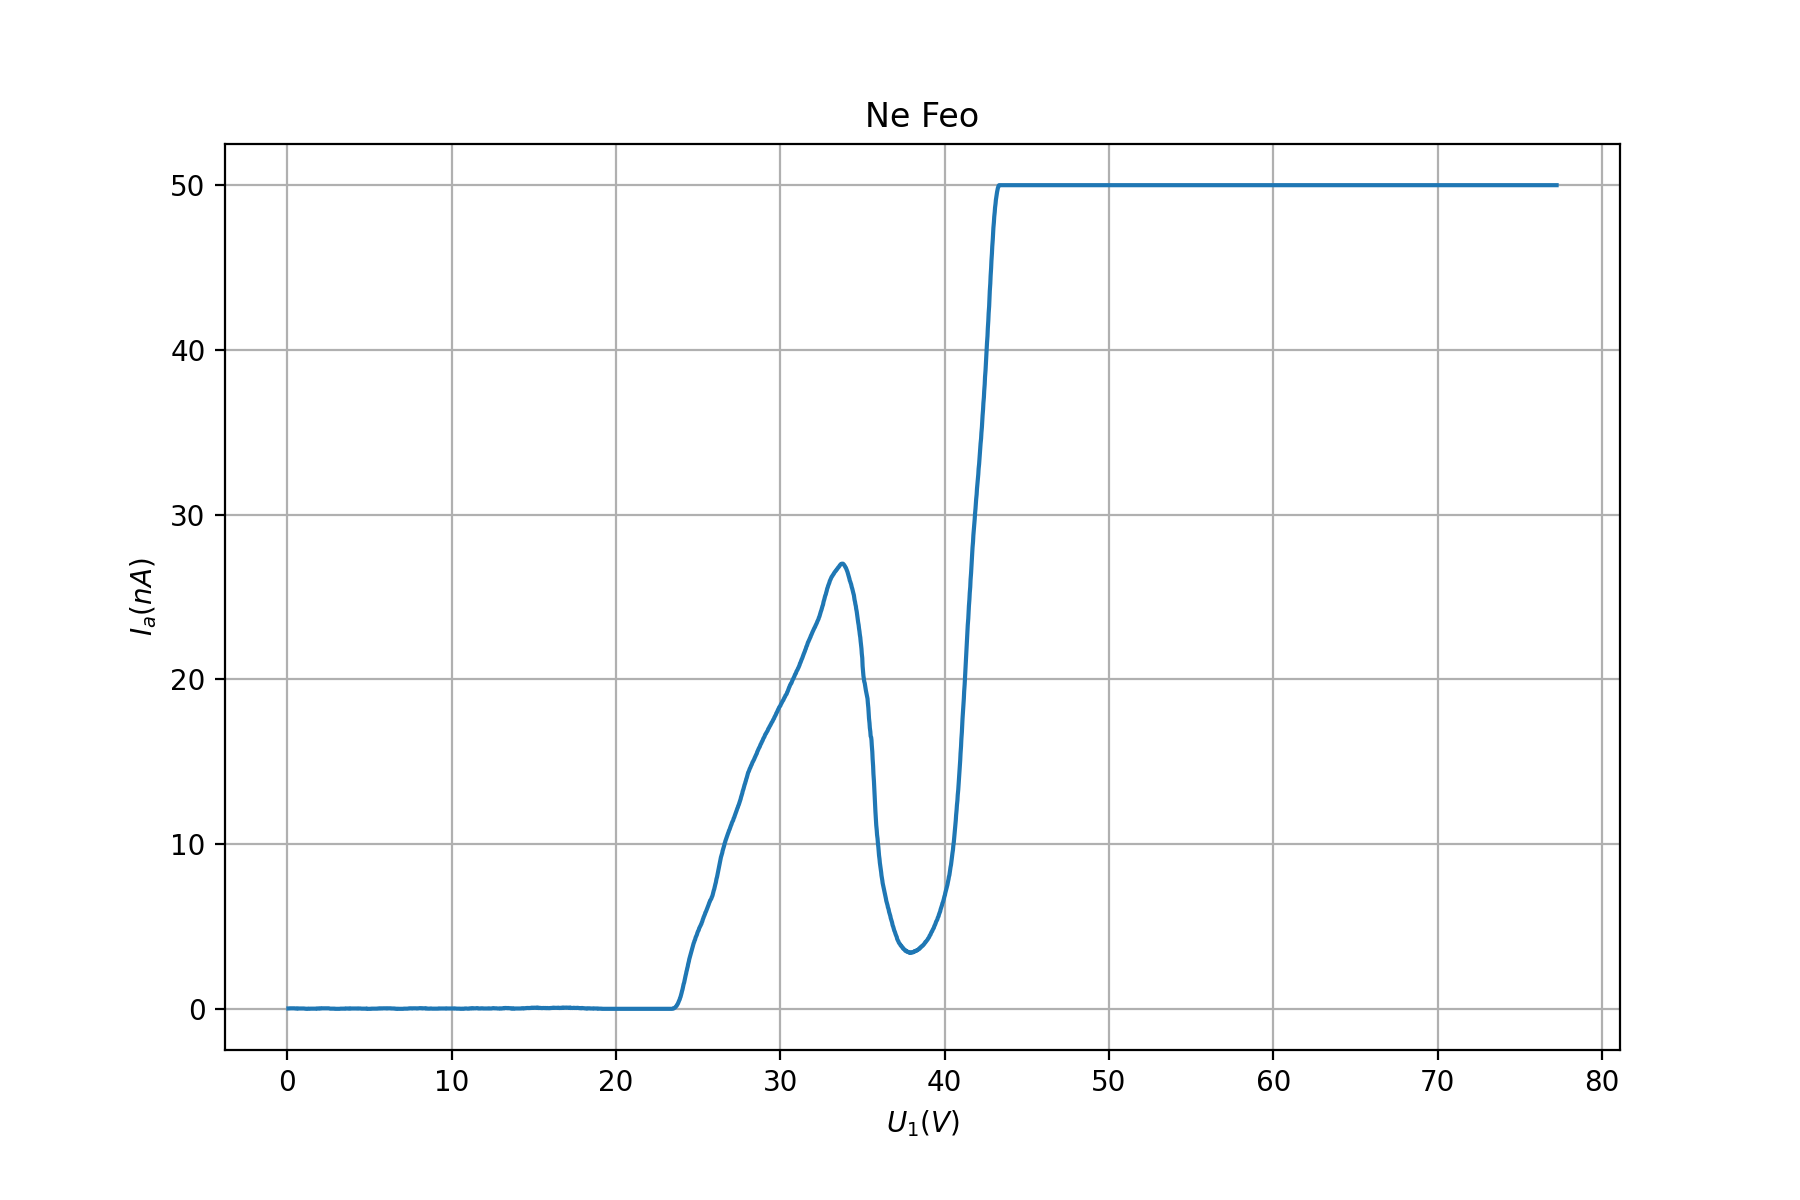
\includegraphics[max width=0.32\linewidth]{Ne Feo}
\caption{Gráficas para $U_3 = 3,5V$, $U_3 = 3V$ y un caso variando $U_2$ que no salía bien.}
\end{center}
\end{figure}

\printbibliography
\end{document}